\documentclass[twoside,11pt]{article}

% ? Specify used packages
\usepackage{graphicx}        %  Use this one for final production.
% \usepackage[draft]{graphicx} %  Use this one for drafting.
% ? End of specify used packages

\pagestyle{myheadings}

% -----------------------------------------------------------------------------
% ? Document identification
% Fixed part
\newcommand{\stardoccategory}  {Starlink User Note}
\newcommand{\stardocinitials}  {SUN}
\newcommand{\stardocsource}    {sun\stardocnumber}
\newcommand{\stardoccopyright}
{Copyright \copyright\ 2012 University of British Columbia \& the Science \& Technology Facilities Council}

% Variable part - replace [xxx] as appropriate.
\newcommand{\stardocnumber}    {258.2}
\newcommand{\stardocauthors}   {Edward Chapin, Andrew G. Gibb, Tim Jenness, David S. Berry, Douglas Scott \& Remo Tilanus}
\newcommand{\stardocdate}      {30 Aug 2012}
\newcommand{\stardoctitle}     {SMURF -- the Sub-Millimetre User Reduction Facillity}
\newcommand{\stardocversion}   {Version 1.4.1}
\newcommand{\stardocmanual}    {User's Guide}
\newcommand{\stardocabstract}  {

  The Sub-Millimetre User Reduction Facility (SMURF) is a software
  package for reducing data produced by the ACSIS correlater and the
  SCUBA-2 bolometer array on the James Clerk Maxwell Telescope
  (JCMT). This document describes how to use SMURF to process raw
  ACSIS data into data cubes, and raw SCUBA-2 data into images.

}
% ? End of document identification
% -----------------------------------------------------------------------------

% +
%  Name:
%     sun258.tex
%
%  Purpose:
%     Documentation for ACSIS and SCUBA-2 data reduction
%
%  Authors:
%     EC: Edward Chapin (UBC)
%     AGG: Andy Gibb (UBC)
%
%  History:
%     2008-11-14 (EC):
%        Initial version -- based on sun.tex
%     2009-04-15 (AGG):
%        Convert Maria's document to LaTeX
%     2009-07-20 (AGG):
%        Significant updates in time for Nanahope Starlink release
%     2009-07-24 (EC):
%        Updated DIMM section, removed .eps from filenames, other cleanup
%     2009-08-06 (EC):
%        Move/re-size some figures, address some comments from Per Friberg
%     2009-08-26 (AGG):
%        Comments from Douglas, add more references
%     2010-01-08 (AGG):
%        More comments from Douglas, update author list and dates
%     2012-08-30 (RPT):
%        Added section on FIT1D
%     {Add further history here}
%
% -

\newcommand{\stardocname}{\stardocinitials /\stardocnumber}
\markboth{\stardocname}{\stardocname}
\setlength{\textwidth}{160mm}
\setlength{\textheight}{230mm}
\setlength{\topmargin}{-2mm}
\setlength{\oddsidemargin}{0mm}
\setlength{\evensidemargin}{0mm}
\setlength{\parindent}{0mm}
\setlength{\parskip}{\medskipamount}
\setlength{\unitlength}{1mm}

% -----------------------------------------------------------------------------
%  Hypertext definitions.
%  ======================
%  These are used by the LaTeX2HTML translator in conjunction with star2html.

%  Comment.sty: version 2.0, 19 June 1992
%  Selectively in/exclude pieces of text.
%
%  Author
%    Victor Eijkhout                                      <eijkhout@cs.utk.edu>
%    Department of Computer Science
%    University Tennessee at Knoxville
%    104 Ayres Hall
%    Knoxville, TN 37996
%    USA

%  Do not remove the %begin{latexonly} and %end{latexonly} lines (used by
%  LaTeX2HTML to signify text it shouldn't process).
%begin{latexonly}
\makeatletter
\def\makeinnocent#1{\catcode`#1=12 }
\def\csarg#1#2{\expandafter#1\csname#2\endcsname}

\def\ThrowAwayComment#1{\begingroup
    \def\CurrentComment{#1}%
    \let\do\makeinnocent \dospecials
    \makeinnocent\^^L% and whatever other special cases
    \endlinechar`\^^M \catcode`\^^M=12 \xComment}
{\catcode`\^^M=12 \endlinechar=-1 %
 \gdef\xComment#1^^M{\def\test{#1}
      \csarg\ifx{PlainEnd\CurrentComment Test}\test
          \let\html@next\endgroup
      \else \csarg\ifx{LaLaEnd\CurrentComment Test}\test
            \edef\html@next{\endgroup\noexpand\end{\CurrentComment}}
      \else \let\html@next\xComment
      \fi \fi \html@next}
}
\makeatother

\def\includecomment
 #1{\expandafter\def\csname#1\endcsname{}%
    \expandafter\def\csname end#1\endcsname{}}
\def\excludecomment
 #1{\expandafter\def\csname#1\endcsname{\ThrowAwayComment{#1}}%
    {\escapechar=-1\relax
     \csarg\xdef{PlainEnd#1Test}{\string\\end#1}%
     \csarg\xdef{LaLaEnd#1Test}{\string\\end\string\{#1\string\}}%
    }}

%  Define environments that ignore their contents.
\excludecomment{comment}
\excludecomment{rawhtml}
\excludecomment{htmlonly}

%  Hypertext commands etc. This is a condensed version of the html.sty
%  file supplied with LaTeX2HTML by: Nikos Drakos <nikos@cbl.leeds.ac.uk> &
%  Jelle van Zeijl <jvzeijl@isou17.estec.esa.nl>. The LaTeX2HTML documentation
%  should be consulted about all commands (and the environments defined above)
%  except \xref and \xlabel which are Starlink specific.

\newcommand{\htmladdnormallinkfoot}[2]{#1\footnote{#2}}
\newcommand{\htmladdnormallink}[2]{#1}
\newcommand{\htmladdimg}[1]{}
\newcommand{\hyperref}[4]{#2\ref{#4}#3}
\newcommand{\htmlref}[2]{#1}
\newcommand{\htmlimage}[1]{}
\newcommand{\htmladdtonavigation}[1]{}

\newenvironment{latexonly}{}{}
\newcommand{\latex}[1]{#1}
\newcommand{\html}[1]{}
\newcommand{\latexhtml}[2]{#1}
\newcommand{\HTMLcode}[2][]{}

%  Starlink cross-references and labels.
\newcommand{\xref}[3]{#1}
\newcommand{\xlabel}[1]{}

%  LaTeX2HTML symbol.
\newcommand{\latextohtml}{\LaTeX2\texttt{HTML}}

%  Define command to re-centre underscore for Latex and leave as normal
%  for HTML (severe problems with \_ in tabbing environments and \_\_
%  generally otherwise).
\renewcommand{\_}{\texttt{\symbol{95}}}

% -----------------------------------------------------------------------------
%  Debugging.
%  =========
%  Remove % on the following to debug links in the HTML version using Latex.

% \newcommand{\hotlink}[2]{\fbox{\begin{tabular}[t]{@{}c@{}}#1\\\hline{\footnotesize #2}\end{tabular}}}
% \renewcommand{\htmladdnormallinkfoot}[2]{\hotlink{#1}{#2}}
% \renewcommand{\htmladdnormallink}[2]{\hotlink{#1}{#2}}
% \renewcommand{\hyperref}[4]{\hotlink{#1}{\S\ref{#4}}}
% \renewcommand{\htmlref}[2]{\hotlink{#1}{\S\ref{#2}}}
% \renewcommand{\xref}[3]{\hotlink{#1}{#2 -- #3}}
%end{latexonly}
% -----------------------------------------------------------------------------
% ? Document specific \newcommand or \newenvironment commands.

% A new environment for quoting verbatim
% Environment for indenting and using a small font.
\newenvironment{myquote}{\begin{quote}\begin{small}}{\end{small}\end{quote}}

\newcommand{\starlink}{\htmladdnormallink{Starlink}{http://starlink.jach.hawaii.edu}}

% Shorthand and HTML references for other Starlink tasks
\newcommand{\CCDPACK}{\textsc{ccdpack}}
\newcommand{\CCDPACKref}{\xref{\CCDPACK}{sun139}{}}
\newcommand{\GAIA}{\textsc{gaia}}
\newcommand{\GAIAref}{\xref{\GAIA}{sun214}{}}
\newcommand{\HDSTRACE}{\textsc{hdstrace}}
\newcommand{\HDSTRACEref}{\xref{\HDSTRACE}{sun102}{}}
\newcommand{\KAPPA}{\textsc{kappa}}
\newcommand{\CURSA}{\xref{\textsc{cursa}}{sun190}{}}
\newcommand{\KAPPAref}{\xref{(SUN/95)}{sun95}{}}
\newcommand{\SMURF}{\textsc{smurf}}
\newcommand{\SMURFcook}{\xref{SC/19}{sc19}{}}
\newcommand{\ADAMsgref}{\xref{SG/4}{sg4}{}}
\newcommand{\ADAMsunref}{\xref{SUN/101}{sun101}{}}
\newcommand{\astref}{\xref{SUN/211}{sun211}{}}
\newcommand{\ndfref}{\xref{SUN/33}{sun33}{}}

% Application tasks
\newcommand{\task}[1]{\textsf{#1}}

% SMURF tasks
\newcommand{\badbolos}{\xref{\task{badbolos}}{sun258}{BADBOLOS}}
\newcommand{\calcdark}{\xref{\task{calcdark}}{sun258}{CALCDARK}}
\newcommand{\calcflat}{\xref{\task{calcflat}}{sun258}{CALCFLAT}}
\newcommand{\calcnoise}{\xref{\task{calcnoise}}{sun258}{CALCNOISE}}
\newcommand{\calcresp}{\xref{\task{calcresp}}{sun258}{CALCRESP}}
\newcommand{\copyflat}{\xref{\task{copyflat}}{sun258}{COPYFLAT}}
\newcommand{\dreamsolve}{\xref{\task{dreamsolve}}{sun258}{DREAMSOLVE}}
\newcommand{\dreamweights}{\xref{\task{dreamweights}}{sun258}{DREAMWEIGHTS}}
%  ...use fitdd instead of fit1d because the 1 breaks the macro
\newcommand{\fitdd}{\xref{\task{fit1d}}{sun258}{FIT1D}}
\newcommand{\gsdtoacsis}{\xref{\task{gsd2acsis}}{sun258}{GSD2ACSIS}}
\newcommand{\gsdshow}{\xref{\task{gsdshow}}{sun258}{GSDSHOW}}
\newcommand{\smurfhelp}{\xref{\task{smurfhelp}}{sun258}{SMURFHELP}}
\newcommand{\impaztec}{\xref{\task{impaztec}}{sun258}{IMPAZTEC}}
\newcommand{\makecube}{\xref{\task{makecube}}{sun258}{MAKECUBE}}
\newcommand{\rawunpress}{\xref{\task{rawunpress}}{sun258}{RAWUNPRESS}}
\newcommand{\rawfixmeta}{\xref{\task{rawfixmeta}}{sun258}{RAWFIXMETA}}
\newcommand{\sctwosim}{\xref{\task{sc2sim}}{sun258}{SC2SIM}}
\newcommand{\sctwothreadtest}{\xref{\task{sc2threadtest}}{sun258}{SC2THREADTEST}}
\newcommand{\scanfit}{\xref{\task{scanfit}}{sun258}{SCANFIT}}
\newcommand{\skynoise}{\xref{\task{skynoise}}{sun258}{SKYNOISE}}
\newcommand{\smurfcopy}{\xref{\task{smurfcopy}}{sun258}{SMURFCOPY}}
\newcommand{\stackframes}{\xref{\task{stackframes}}{sun258}{STACKFRAMES}}
\newcommand{\starecalc}{\xref{\task{starecalc}}{sun258}{STARECALC}}
\newcommand{\timesort}{\xref{\task{timesort}}{sun258}{TIMESORT}}
\newcommand{\unmakecube}{\xref{\task{unmakecube}}{sun258}{UNMAKECUBE}}

\newcommand{\extinction}{\xref{\task{extinction}}{sun258}{EXTINCTION}}
\newcommand{\flatfield}{\xref{\task{flatfield}}{sun258}{FLATFIELD}}
\newcommand{\jcmtstate}{\xref{\task{jcmtstate2cat}}{sun258}{JCMTSTATE2CAT}}
\newcommand{\dumpocscfg}{\xref{\task{dumpocscfg}}{sun258}{DUMPOCSCFG}}
\newcommand{\makemap}{\xref{\task{makemap}}{sun258}{MAKEMAP}}
\newcommand{\gettsys}{\xref{\task{gettsys}}{sun258}{GETTSYS}}

\newcommand{\remsky}{\xref{\task{remsky}}{sun258}{REMSKY}}
\newcommand{\clean}{\xref{\task{sc2clean}}{sun258}{SC2CLEAN}}
\newcommand{\concat}{\xref{\task{sc2concat}}{sun258}{SC2CONCAT}}
\newcommand{\fft}{\xref{\task{sc2fft}}{sun258}{SC2FFT}}
\newcommand{\fts}{\xref{\task{sc2fts}}{sun258}{SC2FTS}}

\newcommand{\rebin}{\texttt{rebin}}
\newcommand{\iterate}{\texttt{iterate}}

% Other tasks
\newcommand{\makemos}{\xref{\task{makemos}}{sun139}{MAKEMOS}}
\newcommand{\csub}{\xref{\task{csub}}{sun95}{CSUB}}
\newcommand{\clinplot}{\xref{\task{clinplot}}{sun95}{CLINPLOT}}
\newcommand{\mlinplot}{\xref{\task{mlinplot}}{sun95}{MLINPLOT}}
\newcommand{\collapse}{\xref{\task{collapse}}{sun95}{COLLAPSE}}
\newcommand{\fitsedit}{\xref{\task{fitsedit}}{sun95}{FITSEDIT}}
\newcommand{\kapdiv}{\xref{\task{div}}{sun95}{DIV}}
\newcommand{\ndfcopy}{\xref{\task{ndfcopy}}{sun95}{NDFCOPY}}
\newcommand{\provshow}{\xref{\task{provshow}}{sun95}{PROVSHOW}}
\newcommand{\thresh}{\xref{\task{thresh}}{sun95}{THRESH}}
\newcommand{\wcsmosaic}{\xref{\task{wcsmosaic}}{sun95}{WCSMOSAIC}}
\newcommand{\wcsalign}{\xref{\task{wcsalign}}{sun95}{WCSALIGN}}
\newcommand{\wcsattrib}{\xref{\task{wcsattrib}}{sun95}{WCSATTRIB}}
\newcommand{\fitslist}{\xref{\task{fitslist}}{sun95}{FITSLIST}}
\newcommand{\display}{\xref{\task{display}}{sun95}{DISPLAY}}
\newcommand{\topcat}{\xref{\textsc{Topcat}}{sun253}{}}


% macros for typesetting parameters
\newcommand{\aparam}[1]{\texttt{#1}}     % ADAM parameter
\newcommand{\cparam}[1]{\texttt{#1}}     % CONFIG parameter
\newcommand{\ndfcomp}[1]{\texttt{#1}}    % NDF component

%% Definitions imported from SUN/95

% A kind of list item, like description, but with an easily adjustable
% item separation.  Note that the paragraph and fount-size change are
% needed to make the revised \baselinestretch work.
\newlength{\menuwidth}
\newlength{\menuindent}
\newcommand{\menuitem}[2]
  {{\bf #1} \settowidth{\menuwidth}{{\bf #1} }
  \setlength{\menuindent}{-0.5em}
  \addtolength{\menuwidth}{-2\menuwidth}
  \addtolength{\menuwidth}{\textwidth}
  \addtolength{\menuwidth}{\menuindent}
  \hspace{\menuindent}\parbox[t]{\menuwidth}{
  \renewcommand{\baselinestretch}{0.75}\small
  #2 \par \vspace{1.0ex}
  \renewcommand{\baselinestretch}{1.0}\normalsize} \\ }
\begin{htmlonly}
\newcommand{\menuitem}[2]
  {\item [\htmlref{#1}{#1}] #2}
\end{htmlonly}

\newcommand{\classitem}[1]{\item [\htmlref{#1}{#1}]}

% an environment for references (for the SST sstdiytopic command).
\newenvironment{refs}{\vspace{-4ex} % normally 3ex
                      \begin{list}{}{\setlength{\topsep}{0mm}
                                     \setlength{\partopsep}{0mm}
                                     \setlength{\itemsep}{0mm}
                                     \setlength{\parsep}{0mm}
                                     \setlength{\leftmargin}{1.5em}
                                     \setlength{\itemindent}{-\leftmargin}
                                     \setlength{\labelsep}{0mm}
                                     \setlength{\labelwidth}{0mm}}
                    }{\end{list}}

%+
%  Name:
%     SST.TEX

%  Purpose:
%     Define LaTeX commands for laying out Starlink routine descriptions.

%  Language:
%     LaTeX

%  Type of Module:
%     LaTeX data file.

%  Description:
%     This file defines LaTeX commands which allow routine documentation
%     produced by the SST application PROLAT to be processed by LaTeX and
%     by LaTeX2html. The contents of this file should be included in the
%     source prior to any statements that make of the sst commnds.

%  Notes:
%     The style file html.sty provided with LaTeX2html needs to be used.
%     This must be before this file.

%  Authors:
%     RFWS: R.F. Warren-Smith (STARLINK)
%     PDRAPER: P.W. Draper (Starlink - Durham University)

%  History:
%     10-SEP-1990 (RFWS):
%        Original version.
%     10-SEP-1990 (RFWS):
%        Added the implementation status section.
%     12-SEP-1990 (RFWS):
%        Added support for the usage section and adjusted various spacings.
%     8-DEC-1994 (PDRAPER):
%        Added support for simplified formatting using LaTeX2html.
%     21-JUL-2009 (TIMJ):
%        Added \sstdiylist{}{} as used when a Parameters section is located that
%        is not "ADAM Parameters".
%     {enter_further_changes_here}

%  Bugs:
%     {note_any_bugs_here}

%-

%  Define length variables.
\newlength{\sstbannerlength}
\newlength{\sstcaptionlength}
\newlength{\sstexampleslength}
\newlength{\sstexampleswidth}

%  Define a \tt font of the required size.
\latex{\newfont{\ssttt}{cmtt10 scaled 1095}}
\html{\newcommand{\ssttt}{\tt}}

%  Define a command to produce a routine header, including its name,
%  a purpose description and the rest of the routine's documentation.
\newcommand{\sstroutine}[3]{
   \goodbreak
   \rule{\textwidth}{0.5mm}
   \vspace{-7ex}
   \newline
   \settowidth{\sstbannerlength}{{\Large {\bf #1}}}
   \setlength{\sstcaptionlength}{\textwidth}
   \setlength{\sstexampleslength}{\textwidth}
   \addtolength{\sstbannerlength}{0.5em}
   \addtolength{\sstcaptionlength}{-2.0\sstbannerlength}
   \addtolength{\sstcaptionlength}{-5.0pt}
   \settowidth{\sstexampleswidth}{{\bf Examples:}}
   \addtolength{\sstexampleslength}{-\sstexampleswidth}
   \parbox[t]{\sstbannerlength}{\flushleft{\Large {\bf #1}}}
   \parbox[t]{\sstcaptionlength}{\center{\Large #2}}
   \parbox[t]{\sstbannerlength}{\flushright{\Large {\bf #1}}}
   \begin{description}
      #3
   \end{description}
}

%  Format the description section.
\newcommand{\sstdescription}[1]{\item[Description:] #1}

%  Format the usage section.
\newcommand{\sstusage}[1]{\item[Usage:] \mbox{}
\\[1.3ex]{\raggedright \ssttt #1}}

%  Format the invocation section.
\newcommand{\sstinvocation}[1]{\item[Invocation:]\hspace{0.4em}{\tt #1}}

%  Format the arguments section.
\newcommand{\sstarguments}[1]{
   \item[Arguments:] \mbox{} \\
   \vspace{-3.5ex}
   \begin{description}
      #1
   \end{description}
}

%  Format the returned value section (for a function).
\newcommand{\sstreturnedvalue}[1]{
   \item[Returned Value:] \mbox{} \\
   \vspace{-3.5ex}
   \begin{description}
      #1
   \end{description}
}

%  Format the parameters section (for an application).
\newcommand{\sstparameters}[1]{
   \item[Parameters:] \mbox{} \\
   \vspace{-3.5ex}
   \begin{description}
      #1
   \end{description}
}

%  Format the examples section.
\newcommand{\sstexamples}[1]{
   \item[Examples:] \mbox{} \\
   \vspace{-3.5ex}
   \begin{description}
      #1
   \end{description}
}

%  Define the format of a subsection in a normal section.
\newcommand{\sstsubsection}[1]{ \item[{#1}] \mbox{} \\}

%  Define the format of a subsection in the examples section.
\newcommand{\sstexamplesubsection}[2]{\sloppy
\item[\parbox{\sstexampleslength}{\ssttt #1}] \mbox{} \vspace{1.0ex}
\\ #2 }

%  Format the notes section.
\newcommand{\sstnotes}[1]{\item[Notes:] \mbox{} \\[1.3ex] #1}

%  Provide a general-purpose format for additional (DIY) sections.
\newcommand{\sstdiytopic}[2]{\item[{\hspace{-0.35em}#1\hspace{-0.35em}:}]
\mbox{} \\[1.3ex] #2}

%  Format the a generic section as a list
\newcommand{\sstdiylist}[2]{
   \item[#1:] \mbox{} \\
   \vspace{-3.5ex}
   \begin{description}
      #2
   \end{description}
}

%  Format the implementation status section.
\newcommand{\sstimplementationstatus}[1]{
   \item[{Implementation Status:}] \mbox{} \\[1.3ex] #1}

%  Format the bugs section.
\newcommand{\sstbugs}[1]{\item[Bugs:] #1}

%  Format a list of items while in paragraph mode.
\newcommand{\sstitemlist}[1]{
  \mbox{} \\
  \vspace{-3.5ex}
  \begin{itemize}
     #1
  \end{itemize}
}

%  Define the format of an item.
\newcommand{\sstitem}{\item}

%% Now define html equivalents of those already set. These are used by
%  latex2html and are defined in the html.sty files.
\begin{htmlonly}

%  sstroutine.
   \newcommand{\sstroutine}[3]{
      \subsection{#1\xlabel{#1}-\label{#1}#2}
      \begin{description}
         #3
      \end{description}
   }

%  sstdescription
   \newcommand{\sstdescription}[1]{\item[Description:]
      \begin{description}
         #1
      \end{description}
      \\
   }

%  sstusage
   \newcommand{\sstusage}[1]{\item[Usage:]
      \begin{description}
         {\ssttt #1}
      \end{description}
      \\
   }

%  sstinvocation
   \newcommand{\sstinvocation}[1]{\item[Invocation:]
      \begin{description}
         {\ssttt #1}
      \end{description}
      \\
   }

%  sstarguments
   \newcommand{\sstarguments}[1]{
      \item[Arguments:] \\
      \begin{description}
         #1
      \end{description}
      \\
   }

%  sstreturnedvalue
   \newcommand{\sstreturnedvalue}[1]{
      \item[Returned Value:] \\
      \begin{description}
         #1
      \end{description}
      \\
   }

%  sstparameters
   \newcommand{\sstparameters}[1]{
      \item[Parameters:] \\
      \begin{description}
         #1
      \end{description}
      \\
   }

%  sstexamples
   \newcommand{\sstexamples}[1]{
      \item[Examples:] \\
      \begin{description}
         #1
      \end{description}
      \\
   }

%  sstsubsection
   \newcommand{\sstsubsection}[1]{\item[{#1}]}

%  sstexamplesubsection
   \newcommand{\sstexamplesubsection}[2]{\item[{\ssttt #1}] #2}

%  sstnotes
   \newcommand{\sstnotes}[1]{\item[Notes:] #1 }

%  sstdiytopic
   \newcommand{\sstdiytopic}[2]{\item[{#1}] #2 }

%  sstimplementationstatus
   \newcommand{\sstimplementationstatus}[1]{
      \item[Implementation Status:] #1
   }

%  sstitemlist
   \newcommand{\sstitemlist}[1]{
      \begin{itemize}
         #1
      \end{itemize}
      \\
   }
%  sstitem
   \newcommand{\sstitem}{\item}

\end{htmlonly}

%  End of "sst.tex" layout definitions.
%.



% ? End of document specific commands
% -----------------------------------------------------------------------------
%  Title Page.
%  ===========
\renewcommand{\thepage}{\roman{page}}
\begin{document}
\thispagestyle{empty}

%  Latex document header.
%  ======================
\begin{latexonly}
   \textsc{University of British Columbia} / \textsc{Joint Astronomy Centre} \hfill \textbf{\stardocname}\\
   {\large Science \& Technology Facilities Council}\\
   {\large Starlink Software Collection\\}
   {\large \stardoccategory\ \stardocnumber}
   \begin{flushright}
   \stardocauthors\\
   \stardocdate
   \end{flushright}
   \vspace{-4mm}
   \rule{\textwidth}{0.5mm}
   \vspace{5mm}
   \begin{center}
   {\Huge\textbf{\stardoctitle \\ [2.5ex]}}
   {\LARGE\textbf{\stardocversion \\ [4ex]}}
   {\Huge\textbf{\stardocmanual}}
   \end{center}
   \vspace{5mm}

% ? Add picture here if required for the LaTeX version.
%   e.g. \includegraphics[scale=0.3]{filename.ps}
\begin{center}
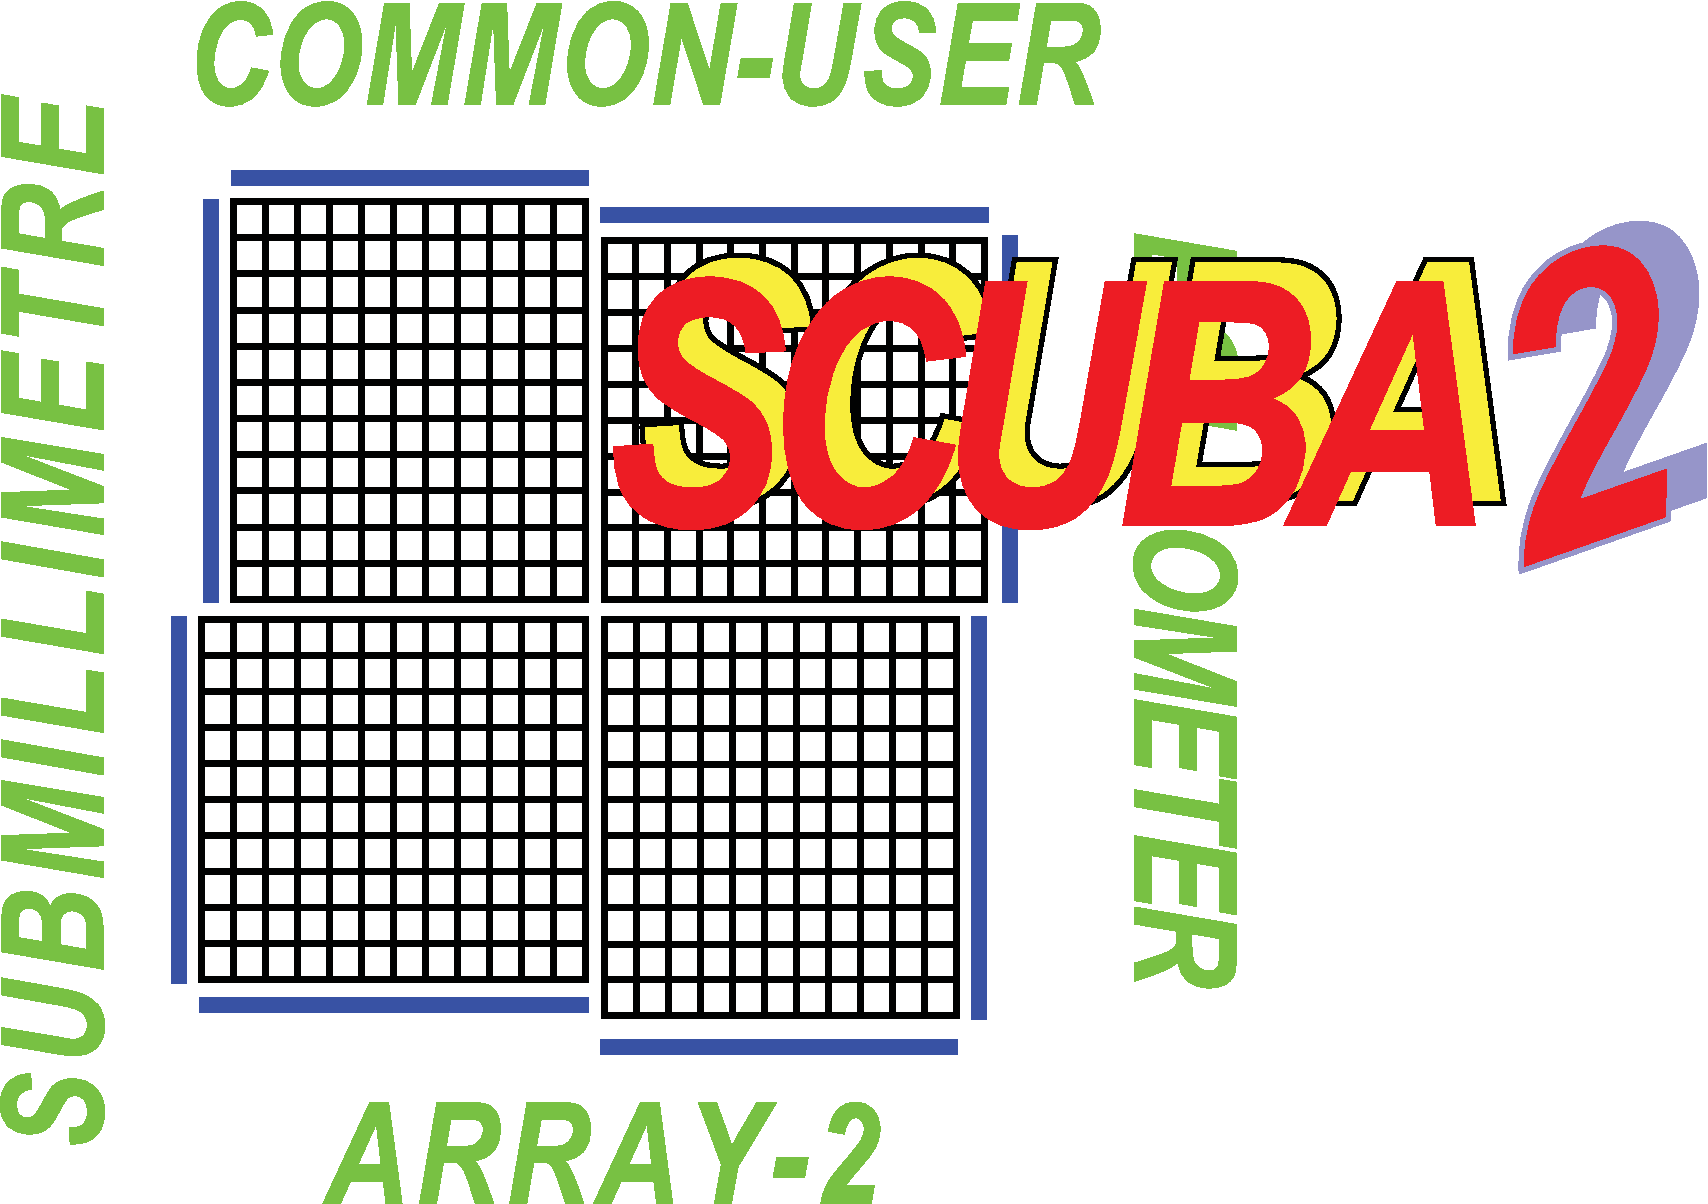
\includegraphics[scale=0.3]{sun258_logo}
\end{center}
% ? End of picture

% ? Heading for abstract if used.
   \vspace{10mm}
   \begin{center}
      {\Large\textbf{Abstract}}
   \end{center}
% ? End of heading for abstract.
\end{latexonly}

%  HTML documentation header.
%  ==========================
\begin{htmlonly}
   \xlabel{}
   \begin{rawhtml} <H1> \end{rawhtml}
      \stardoctitle\\
      \stardocversion\\
      \stardocmanual
   \begin{rawhtml} </H1> <HR> \end{rawhtml}

% ? Add picture here if required for the hypertext version.
%   e.g. \includegraphics[scale=0.7]{filename.ps}
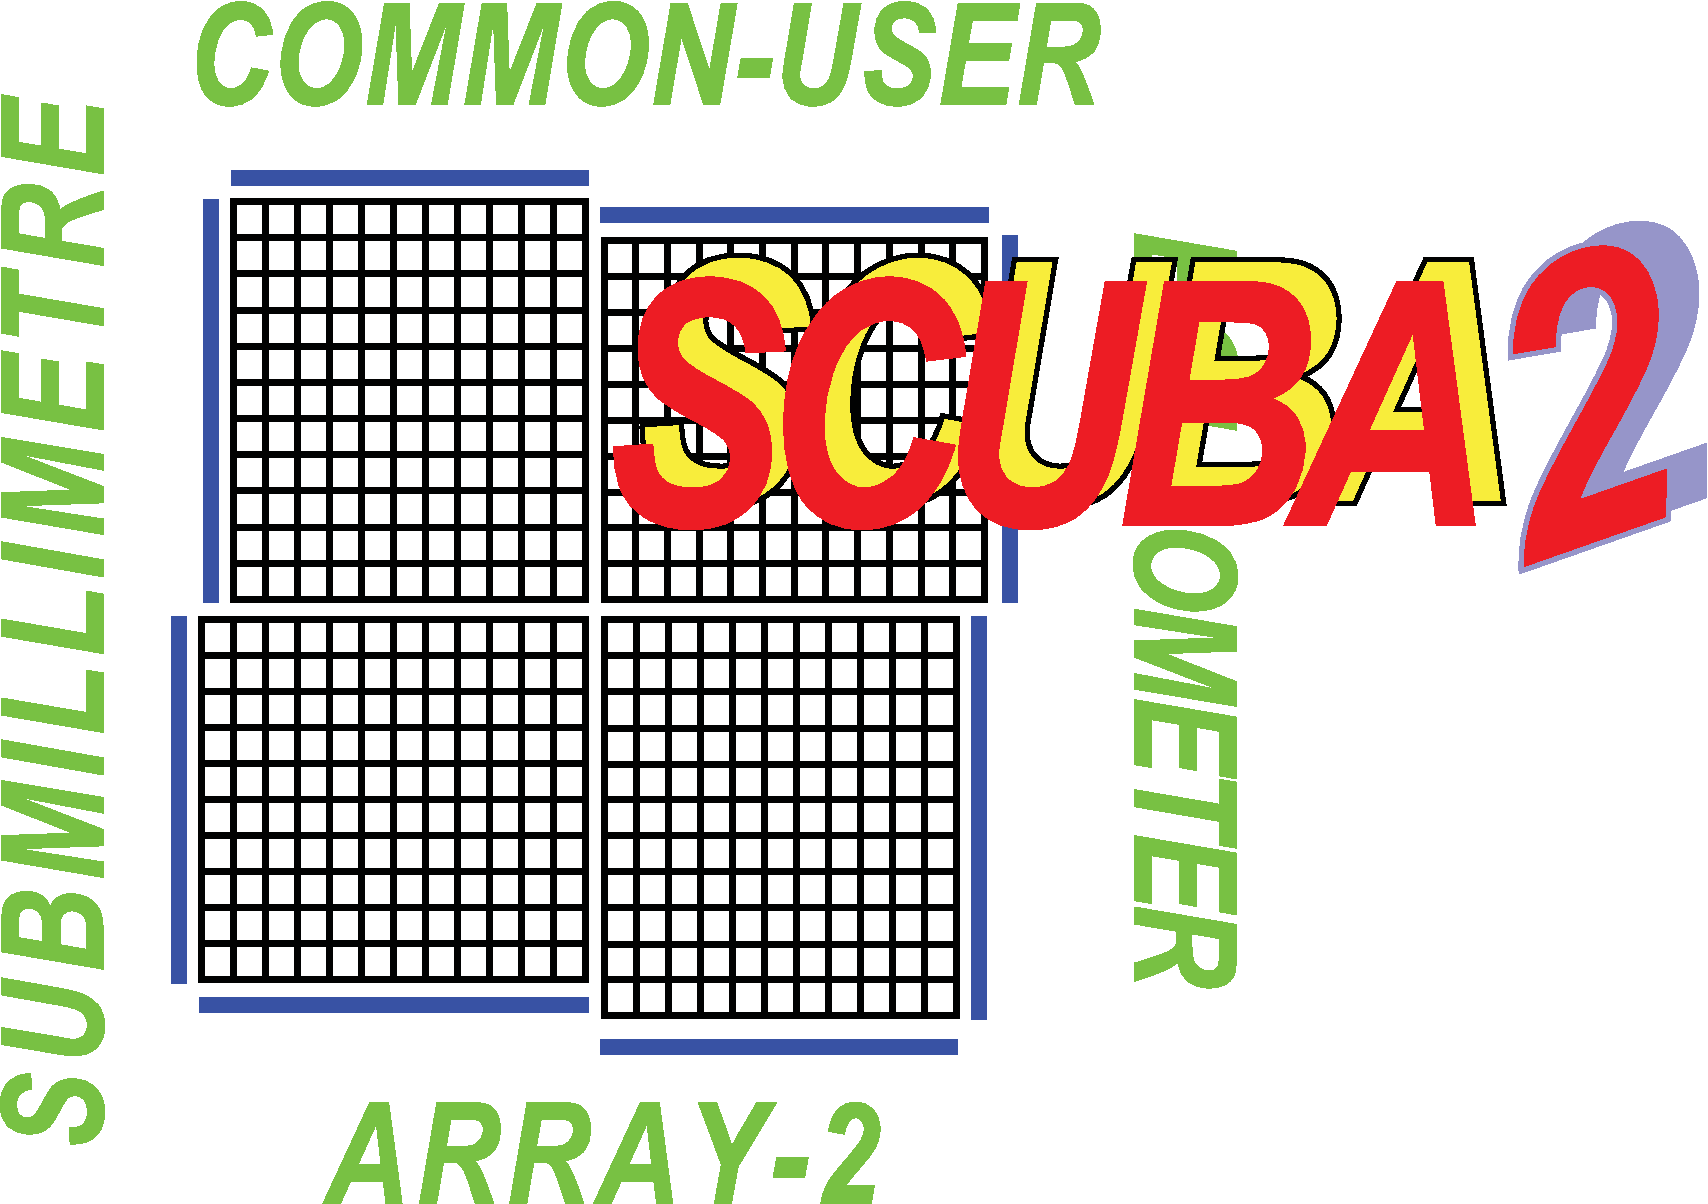
\includegraphics[scale=0.7]{sun258_logo}
% ? End of picture

   \begin{rawhtml} <P> <I> \end{rawhtml}
   \stardoccategory\ \stardocnumber \\
   \stardocauthors \\
   \stardocdate
   \begin{rawhtml} </I> </P> <H3> \end{rawhtml}
      \htmladdnormallink{University of British Columbia}
                        {http://www.ubc.ca} \\
      \htmladdnormallink{Joint Astronomy Centre}
                        {http://www.jach.hawaii.edu}\\
      \htmladdnormallink{Science \& Technology Facilities Council}
                        {http://www.stfc.ac.uk} \\
   \begin{rawhtml} </H3> <H2> \end{rawhtml}
      \htmladdnormallink{Starlink Software Collection}{http://starlink.jach.hawaii.edu/}
   \begin{rawhtml} </H2> \end{rawhtml}
   \htmladdnormallink{\htmladdimg{source.gif} Retrieve hardcopy}
      {http://starlink.jach.hawaii.edu/cgi-bin/hcserver?\stardocsource}\\

%  HTML document table of contents.
%  ================================
%  Add table of contents header and a navigation button to return to this
%  point in the document (this should always go before the abstract \section).
  \label{stardoccontents}
  \begin{rawhtml}
    <HR>
    <H2>Contents</H2>
  \end{rawhtml}
  \htmladdtonavigation{\htmlref{\htmladdimg{contents_motif.gif}}
        {stardoccontents}}

% ? New section for abstract if used.
  \section{\xlabel{abstract}Abstract}
% ? End of new section for abstract
\end{htmlonly}

% -----------------------------------------------------------------------------
% ? Document Abstract. (if used)
%  ==================
\stardocabstract
% ? End of document abstract

% -----------------------------------------------------------------------------
% ? Latex Copyright Statement
%  =========================
\begin{latexonly}
\newpage
\vspace*{\fill}
\stardoccopyright
\end{latexonly}
% ? End of Latex copyright statement

% -----------------------------------------------------------------------------
% ? Latex document Table of Contents (if used).
%  ===========================================
  \newpage
  \begin{latexonly}
    \setlength{\parskip}{0mm}
    \tableofcontents
    \setlength{\parskip}{\medskipamount}
    \markboth{\stardocname}{\stardocname}
  \end{latexonly}
% ? End of Latex document table of contents
% -----------------------------------------------------------------------------

\cleardoublepage
\renewcommand{\thepage}{\arabic{page}}
\setcounter{page}{1}

% Main text

\section{\xlabel{introduction}Introduction\label{se:smurfintro}}

This guide is divided into two main parts, one dedicated to processing
ACSIS data (\cite{acsis}, see Section \ref{se:acsisdr}) and the other
for processing SCUBA-2 data (\cite{scuba2}, see Section
\ref{se:sc2dr}). This first section will introduce \SMURF\ and the
basics of operation. The SMURF Cookbook (\SMURFcook) is also
available, providing an introduction to SCUBA-2 data processing.

\SMURF\ is a suite of \starlink\ ADAM tasks (\xref{SUN/101}{sun101}{}
and \xref{SG/4}{sg4}{}) and therefore requires the \starlink\
environment to be defined.

\subsection{Document conventions}

In an attempt to make this document clearer to read, different fonts
are used for specific structures.

Observing modes are denoted by all upper case body text (e.g.\
FLATFIELD).

Starlink package names are shown in small caps (e.g.\ \SMURF);
individual task names are shown in sans-serif (e.g.\ \makemap).

Content listings are shown in fixed-width type (sometimes called
`typewriter'). Extensions and components within NDF (\ndfref) data
files are shown in upper case fixed-width type (e.g.\
\ndfcomp{HISTORY}).

Text relating to filenames, key presses or entries typed at the
command line are also denoted by fixed-width type (e.g.\ \texttt{\%
  smurf}), as are parameters for tasks which are displayed in upper
case (e.g.\ \aparam{METHOD}).

References to Starlink documents, i.e., Starlink User Notes (SUN),
Starlink General documents (SG) and Starlink Cookbooks (SC), are given
in the text using the document type and the corresponding number
(e.g.\ SUN/95). Non-Starlink documents are cited in the text and
listed in the bibliography.

\subsection{Using SMURF}

\subsubsection{Starting SMURF}

Enable the \SMURF\ environment by typing \verb+smurf+ at the shell
prompt. The welcome message will appear as shown below:
\begin{myquote}
\begin{verbatim}

        SMURF commands are now available -- (Version 1.0.0)

        Type smurfhelp for help on SMURF commands.
        Type 'showme sun258' to browse the hypertext documentation.

        NOTE, several applications have had major changes made to their
        parameter lists. See the 'Release Notes' section of SUN/258 for
        details.

\end{verbatim}
\end{myquote}
This defines aliases for each \SMURF\ command, gives a reminder of the
help command and shows the version number. You can now use \SMURF\
routines or ask for help.

\subsubsection{Getting help}

Access the \SMURF\ online help system as follows:
\begin{enumerate}
\item At the prompt, type \smurfhelp. The welcome message is
  displayed along with a list of available topics.
\item To get information, type the name of an available topic at the
  help prompt.  The next level of help lists information and further
  subtopics.
\item To go to the next level, type the name of a subtopic.
\item Type a question mark, \verb+?+, to re-display the available
  topics at the current level.
\item To go back one level, press \verb+<Enter>+.
\item To exit the help system, press \verb+<Enter>+ until you return
  to the shell prompt.
\end{enumerate}
Further help on the help system maybe obtained by accessing the topic
\verb+smurfhelp+ from within \smurfhelp. If you know which topic you
want help on you can access it directly using

\begin{myquote}
\begin{verbatim}
% smurfhelp makemap parameters
\end{verbatim}
\end{myquote}

If an application prompts you for input and you do not know what the
parameter means, you can use \verb+?+ at the prompt for more
information.

\begin{myquote}
\begin{verbatim}
% calcflat
IN - Input flatfield files > ?

CALCFLAT

  Parameters

    IN

      IN = NDF (Read)
         Input files to be processed. Must all be from the same
         observation and the same subarray.

IN - Input flatfield files >
\end{verbatim}
\end{myquote}

\subsubsection{SMURF parameters}

\SMURF\ uses named parameters to specify input and output files and
other variables necessary for data processing. \KAPPA\ \KAPPAref\ has a
convenient overview of the parameter system used by \SMURF.

\subsubsection{Message filter}

All \SMURF\ commands support the `message filter' parameter
(\verb+msg_filter+), which controls the number of messages \SMURF\
writes to the screen when executing routines. The default setting for
the message filter is \verb+normal+. Table \ref{tab:msgfilter} lists
the available values for \verb+msg_filter+. Be aware that specifying
\verb+verbose+ or \verb+debug+ will slow down execution due to the
(potentially vast) number of messages written to the terminal. It is
also possible to control message output by setting the
\verb+MSG_FILTER+ environment variable to one of the values listed in
this table. To hide all message a quick option is to add \verb+QUIET+
to the command line.

\begin{table}
\centering
\begin{tabular}{|c|l|}
\hline
Option  & Description \\
\hline
none    & No messages \\
quiet   & Limited messages \\
normal  & Very few messages \\
verbose & Full messages \\
debug   & Some debugging messages (useful for programmers) \\
all     & All messages regardless of debug level \\
\hline
\end{tabular}
\label{tab:msgfilter}
\end{table}

\subsubsection{\xlabel{files}Working with data files\label{se:files}}

\SMURF\ does not itself enforce a naming scheme on files. However, raw
data from ACSIS and SCUBA-2 obey a well-defined naming scheme. The
convention is as follows: the name is composed of an instrument
prefix, the UT date in the form YYYYMMDD, a zero-padded five-digit
observation number, followed by a two-digit sub-system number (ACSIS
only) and a zero-padded four-digit subscan number, all separated by
underscore characters. The file has an extension of \verb+.sdf+. The
instrument prefix for ACSIS is simply \verb+a+. For SCUBA-2 it is a
three-character string dependent on the particular subarray from which
the data were recorded. The SCUBA-2 subarrays are labelled a--d at
each wavelength, which are coded by a single digit (either 4 or 8 for
450 and 850\,$\mu$m data respectively); thus the SCUBA-2 prefix is
\verb+s[4|8][a-d]+.

Example ACSIS filename: a20090620\_00023\_01\_0002.sdf\\
Example SCUBA-2 filename: s8a20090620\_00075\_0001.sdf

Files can be processed either singly or in batches. It is more
efficient to process multiple files at the same time. To work with
multiple files you can specify them in a text file using group file
indirection syntax (the `\verb+^+' caret before the filename), using shell
wildcards (escaped from the shell itself) or by listing them
explicitly separated by commas. For more information on specifying
groups of objects for input and output see \xref{the section
  \textit{Specifying Groups of Objects} in
  SUN/95}{sun95}{se_groups}. Examples of valid inputs are:
\begin{myquote}
\begin{verbatim}
IN=s8a20090620_00075_0001.sdf
IN=s8a20090620_00075_*
IN=s8a20090620_00075_00??
IN=file1,file2
IN=^myfile.lis
OUT=*_out
\end{verbatim}
\end{myquote}

Note that if you are providing a text file containing output
filenames, those should be listed in the same order as the input
filenames, otherwise the processed data will be written under
the wrong filenames. Take care to supply a different output file name
from the input as the contents are overwritten!

\subsection{Data file structure}

Data files for both ACSIS and SCUBA-2 \cite{sc2ic01} use the Starlink N-Dimensional
data format (NDF, see \ndfref), a hierarchical format which allows
additional data and metadata to be stored within a single file. Raw
files contain a number of NDF components which store
observation-specific data necessary for subsequent processing. The
contents of these (and other NDF) files may be listed with
\HDSTRACEref. Each file on disk is also known as a `subscan'.

The main (top-level) components are:
\begin{itemize}
\item Raw data (a 3-dimensional array);
\item World Coordinate System information;
\item History;
\item Raw data units (K for ACSIS, adu (possibly as compressed integers) for raw SCUBA-2 data,
  pW for flatfielded SCUBA-2 data).
\end{itemize}
For ACSIS, the raw data are stored as $N_{\rm chan} \times N_{\rm
  receptors} \times N_{\rm samp}$, while SCUBA-2 data are stored as
$N_{\rm columns} \times N_{\rm rows} \times N_{\rm samp}$, where
$N_{\rm samp}$ is the number of time samples in a file.

The files also contain additional NDF components common to both
instruments:
\begin{itemize}
\item JCMT State structure (the telescope pointing record) and other
  metadata that potentially varies for every sample;
\item JCMT Observatory Control System (OCS) configuration, with the
  contents of the XML file used to set up the observation;
\item Flexible Image Transport System (FITS) header containing
  information that does not change during a subscan.
\end{itemize}

The \jcmtstate\ command can be used to extract the time varying
metadata and store it in a tab-separated table
(\xref{TST}{sun190}{ACCESS}) format catalogue.\footnote{This is a
  standard format historically supported by \CURSA\ and ESO SkyCat} so
that it can be visualised using \topcat. An example \topcat\ plot of the
telescope motion for a particular observation can be seen in
\ref{fig:topcat}. The JCMTSTATE extension contains information from
the telescope, secondary mirror and real-time sequencer (RTS). ACSIS
observations include environmental weather information and SCUBA-2
observations include SCUBA-2 data (such as the mixing chamber
temperature) and the water vapour monitor (WVM) raw data. \jcmtstate\
converts the telescope and SMU information to additional columns
showing the tracking and AZEL offsets and also converts raw WVM data
to a tau (CSO units). Finally, SCUBA-2 data has additional low-level
MCE information that can be included in the output catalogue using the
`\verb+--with-mce+` option.

\begin{figure}
\begin{center}
\includegraphics{sun258_scan_pattern}
\caption{The telescope positions during observation number 7 on
  20090107. The plot is created by \topcat\ from the output from
\jcmtstate\ plotting the DRA columns against the DDEC column. The pong
scan pattern is clearly visible.}
\label{fig:topcat}
\end{center}
\end{figure}

The original XML used to specify the details of the observation can be
obtained from any data file using the \dumpocscfg\ command.

The FITS header is used to store information that either does not
change or changes by a small amount during the course of an
observation. Note that in the particular case of SCUBA-2 data a
portion of the FITS header will change for each subscan (i.e. file) of
a single observation. The FITS header may be viewed with the \KAPPA\
\fitslist\ command.

Each instrument has further specific components. SCUBA-2 files contain
dark SQUID data, the current flatfield solution, an image of the
bolometers used for heater tracking and possibly information
indicating how to uncompress the raw data. ACSIS files contain
information about the receptors used including their coordinates in
the focal plane.

Output files created by \SMURF\ may contain some or all of these, plus
new components with information about the output data. These are noted
in the description of specific applications. All output files contain
a \ndfcomp{PROVENANCE} extension which provides a detailed record of
the data processing history. Use the \KAPPA\ command \provshow\ to list
the contents.

\subsection{Supported coordinate systems}

\SMURF\ uses AST (\astref) for its astrometry and thus any coordinate
system supported by AST may be used when creating images/cubes. The
default behaviour is to use the same system in which the observations
were made (known as \aparam{TRACKING}).

\subsubsection{Moving sources}

The mapping tasks \makemap\ and \makecube\ automatically
deal with moving sources. There is no need to deal with moving sources
explicitly for any processing with \SMURF. However, mosaicking of
DREAM and STARE images of moving sources will require the WCS
attributes \verb+AlignOffset+ and \verb+SkyRefIs+ to be changed to 1
and `origin' respectively. Use the \KAPPA\ task \wcsattrib\ to
modify these attributes.

\subsection{File sizes and disk space}

Be aware that the raw data files from both instruments may be large
(tens to hundreds of megabytes). Subsequent processing of raw SCUBA-2
time-series data produces output files which are larger due to the
conversion from integer\footnote{Data can be written in either
  \texttt{\_WORD} or \texttt{\_INTEGER} format so the uncompression
  factor can vary from 2 to 4. The \rawunpress\ command can be used to
  uncompress the \texttt{\_WORD} data to \texttt{\_INTEGER} format
  prior to running \flatfield.}  to \verb+_DOUBLE+. \SMURF\ mapping
tasks have the ability to restrict the size of output data files for
manipulation on 32-bit operating systems. See the sections on
\makemap\ and \makecube\ for further details. Processing
SCUBA-2 data is faster on 64-bit systems due to its use of double
precision for all calculations.

\section{\xlabel{acsis}ACSIS Data Reduction\label{se:acsisdr}}

SMURF contains a small number of commands specifically directed towards
the reduction of ACSIS data. This section contains an introduction to
each of these commands. The reduction of ACSIS data is described
more fully in the {\em ACSIS Data Reduction Cookbook}:
\htmladdnormallink{\texttt{http://www.jach.hawaii.edu/JCMT/spectral\_line/data\_reduction/acsisdr/}}
{http://www.jach.hawaii.edu/JCMT/spectral_line/data_reduction/acsisdr/}.

\subsection{The makecube command}

The central step in the reduction of ACSIS data is the conversion of one
or more time-series cubes with {\tt [spectral channel number, receptor
index, time-slice index]} axes, into a spatial cube with {\tt
[RA, Dec, spectral channel number]} axes\footnote{The RA and Dec axes may
be replaced by axes appropriate for other celestial co-ordinate
systems.}. This step is accomplished using the \makecube\ command.

This command first defines the extent (in both pixels and world
co-ordinates) of the output cube, initialises the output cube to hold
zero at every pixel, and then goes through each receptor sample value in
the input data. For each such sample, it first works out its position on
the sky and its spectral position, using the meta-data in the input
files. It then determines the pixel in the output cube that has the same
spatial and spectral position, and then ``pastes'' the sample value into
the output cube at this central pixel position. This pasting involves
dividing the input sample value up between the output pixels in the
neighbourhood of the central output pixel, and then incrementing each of
these output pixel values by its assigned share of the input sample
value. Various schemes can be used to determine the share assigned to each
output pixel - the simplest and fastest is ``nearest neighbour'' in which
the whole input sample value is assigned to the central output pixel.
Whilst being fast, this scheme can produce small geometric shifts in
feature positions. Other available schemes include a bi-linear scheme
that spreads each input value out linearly between the four closest
output pixels, Gaussian weighting with a given radius, Sinc weighting,
{\em etc}.

There are many other aspects of the operation of \makecube\ that can be
controlled via various program parameters, some the more important of
which are:

\begin{itemize}

\item The output data can be split up amongst multiple output cubes, thus
reducing the size of each individual cube.

\item The world co-ordinate system used by the output cubes can be
specified. This includes both the nature of the WCS axes themselves and
the details of the tangent-plane projection (pixel size, orientation,
{\em etc}). If required, optimal values for the projection details can be
determined automatically to produce a regular grid (or as close to a
regular grid as is possible given the input data). Alternatively, the WCS
in the output cube be copied from a specified reference NDF.

\item Output variance values can be calculated either on the basis
of the spread of the input data values that contribute to each output pixel,
or on the basis of the system noise temperature values supplied in the
input NDFs.

\item Input data from specified receptors can be excluded.

\item Input data from specified spectral channels can be excluded.

\item A catalogue can be created holding the spatial position of every
used input sample value.

\end{itemize}

\subsection{The timesort command}

The \makecube\ commands turns time-series cubes into spatial cubes. Each
plane in a time-series cube contains a set of spectra - one for each
used receptor - observed simultaneously at a time given by the position
of the plane on the third axis. It should be noted that the times
associated with this third axis are not guaranteed to increase
monotonically, although that will often be the case. For various reasons,
the writing out of some times slices to the time-series cube may be delayed,
resulting in backwards steps in time along the third axis. This in itself
is not a problem for \makecube\, which makes no assumptions about the
order in which time-slices are stored in the time-series cube. However,
other commands may fail - particularly commands that need to locate the
time-slice index associated with a given time. Such commands assume that
time is a monotonic function of time-slice index, and that therefore the
equivalent of a simple binary chop can be used to locate the index
associated with a given time. These commands will fail with a message
indicating that ``no inverse transformation can be found'' if the
time-series cube contains any out-of-order time slices. Operations that
may produce such a failure include attempting to use \KAPPA\ \wcsalign\
to align two time-series cubes, or displaying a 2D slice of a time-series
cube using \KAPPA\ \display. In these cases, the time-series cube can be
``rectified'' using \timesort. This produces a copy of the cube in which
the time slices are in monotonic order.

In addition, \timesort\ can also be used to assemble and re-order the time
slices from multiple input cubes relating to the same observation, and then
write them out again into a set of time-series cubes, each of a specified
size. In this situation, if a single time slice is split across two
input cubes (which can happen - spectra from some detectors being recorded
in one file and those from the other detectors in another file), they
will be merged together into a single plane in one of the output cubes.


\subsection{The unmakecube command}

The process of converting one or more time-series cubes into a spatial
cube will usually produce some degree of smoothing in the output data due
to multiple input samples contributing to each pixel in the output cube.
This smoothing can sometimes be useful in terms of reducing systematic
differences between the input time-series cubes, such as differing
base-lines. In these cases it is informative to be able to quantify the
effect of this smoothing. The \unmakecube\ command provides this facility
- it creates a set of ``artificial'' time-series cubes from a given
spatial cube. In detail, for each sample position in a given set of input
time-series cubes, a given spatial cube is interpolated to create a new
spectrum, which is then stored at the corresponding position in an output
time-series cube. Thus, any smoothing present in the spatial cube is
transferred into the output time-series cube.

A typical scheme for using unmakecube is:

\begin{enumerate}
\item use makecube to convert a set of ``genuine'' time-series cubes into
a spatial cube.
\item use unmakecube to generate a set of ``artificial'' time-series cubes
from the makecube output spatial cube. The original ``genuine''
time-series cubes are used as templates for the new time-series cubes, so
that they will be aligned sample-for-sample.
\item use the facilities of \KAPPA\ or \GAIA\ to visualise or quantify the
differences between the ``genuine'' and ``artificial'' time-series cubes.
\end{enumerate}

\begin{figure}[htb]
  \begin{center}
    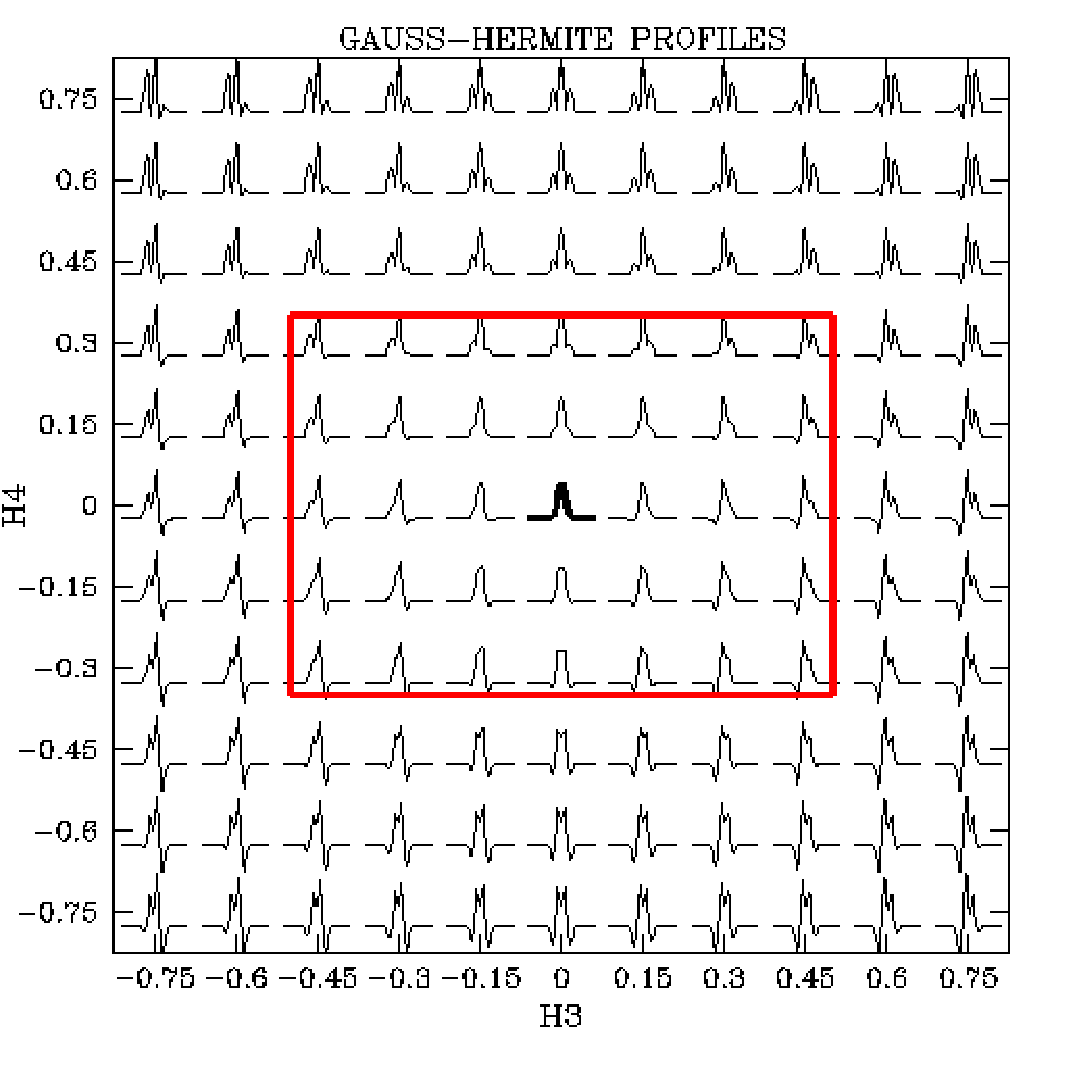
\includegraphics[width=0.8\linewidth]{sun258_gaussherm}
    \caption{Fit1d $-$ Gauss-Hermite shapes as a function of the 3rd-order
      ``skewness'' coefficient h3 and the 4th-order the ``peakiness''
      coefficient h4.  the 3rd-order, h3, and the 4th-order, h4,
      coefficients. The red box indicates the limits on acceptable
      values for h3 and h4 as defined in the defaults config file. Note
      that the fitted profile by default is restricted to positive values
      and this will omit the shown negative features (see
      the \cparam{POS\_ONLY} configuration paramter.}
    \label{fig:gaussherm}
  \end{center}
\end{figure}

\subsection{The fit1d command}

The \fitdd\ command fits profiles along a particular axis of a NDF
data file.  It is a generic command that will work on hypercubes with
upto 7 dimensions, but is here discussed in terms of a typical 3-D
ACSIS data-file with axes RA, Dec, and Vlsr. Specifically, the fitting
of spectra across the imaged section of the sky. The output of \fitdd\
is a cube with the fitted profiles and ``Component parameter files as
NDF extentions''. Be aware that the input cube is expected to be
baseline subtracted and to have a zerolevel of 0.

What sets \fitdd\ apart from most other fitting routines is that, by
using ``Component parameter files'' as inputs, it gives individual
control over the fitting at each position. For instance, it is
possible to fit broad lines on the nucleus of a galaxy but narrow
lines everywhere else in the disk. Or to fit multiple components in an
outflow and single components everywhere else in the field. Still,
these types of fits may require a considerable familiarity with
handling, cutting, and pasting NDF files in order to ``create'' the
desired parameter files for input.

\begin{figure}[htb]
  \begin{center}
    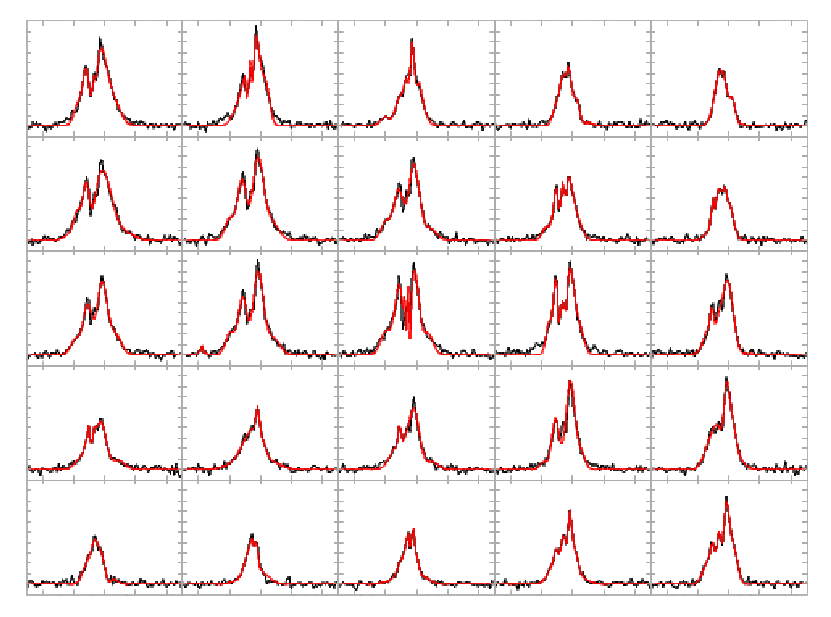
\includegraphics[width=0.8\linewidth]{sun258_fit1d_fits}
    \caption{Fit1d $-$ Black: original profiles; Red: results of a
    3-component Gauss-Hermite2 fit (fitting both h3 and h4, see next section)}
    \label{fig:samplefits}
  \end{center}
\end{figure}

\fitdd\ can also fit more complicated shapes than gaussians. In
particular, gauss-hermite functions are a powerful extention when
fitting profiles that are skewed, peaky, or only approximately
gaussian. Figure \ref{fig:gaussherm} shows gauss-hermite profiles as a
function of the ``skewness'' coefficient h3 and the ``peakiness''
coefficient h4. The red box indicates the limits on acceptable values
for h3 and h4 as defined in the defaults config file. The limits were
chosen such as to exclude fits that look more like multiple components
rather than a distorted single gaussian, but, admittedly are fairly
arbitrary.

Because of the ability to fit distorted shapes, gauss-hermites are
particularly well suited to ``capture'' the maximum amount of emission
from a cube. Figure \ref{fig:samplefits} shows an example of the
quality of the fits that can be obtained. For the shown case \fitdd\
used a 3-component gauss-hermite2 (fitting h3 and h4) function with
the range around the profiles and the remaining configuration
parameters at their default setting.  Collapsing the cube with the
fitted profiles can thus result in an accurate and almost noise-free
white light or total emission map. Residuals from the fit can of
course be studied by subtracting the fitted profiles from the original
cube.

\subsubsection{Fitting functions}

\fitdd\ does a one-dimensional fit along each ``profile'' (spectrum),
fitting the number of requested ``components'' concurrently. Function
shapes that can be fitted are ``gaussians'', ``gausshermite1'',
``gausshermite2'', and ``voigt'' functions, which are discussed in
detail in:

\begin{myquote}
\begin{verbatim}
% smurfhelp fit1d fitting_functions
\end{verbatim}
\end{myquote}

Gauss-hermite profiles are easiest visualized as the combination of a
gaussian and decaying asymmetric 3rd-order and/or symmetric 4th-order
polynomials. The 3rd-order polynomial causes a positive bump on one
side and a negative bump on the other side of the main gaussian,
resulting in asymmetric wings and a skewed shape. By contrast the
4th-order polynomial causes a bump in the centre and steeper slopes
i.e. a peaky shape.

The gauss-hermite profiles in \fitdd\ are called gausshermite1,
fitting only h3, and gausshermite2, fitting both h3 and h4 (to fit
only h4, use gausshermite2 and define h3 to be 0 and fixed). The
default in the configuration file for \cparam{FUNCTION} is a
gausshermite2.

To emphasize a number of issues:

\begin{enumerate}
\item Be aware that the art of fitting profiles is not in the fits
  themselves, but rather the initial estimates provided to the
  fit. Supplying user-defined initial estimates for e.g. the width of
  the profiles can greatly influence and help the resulting fit. Also, if
  the initial estimate routine can only find 2 components, the fit will
  also be restricted to fitting that number of components even if the
  user is requesting more.
\item Setting the configuration parameter \cparam{ESTIMATE\_ONLY} to 1
  will skip the fit and produce an output file with profiles based on the
  initial estimates, allowing the user to inspect those. The associated
  Component parameter files could be modified and used as initial estimates
  for a subsequent fit (see next section).
\item Figure \ref{fig:gaussherm} shows that gauss-hermites can have
  prominent negative features. By default these are set to zero in the
  fitted spectra: see information in the configuration file for the
  parameter \cparam{POS\_ONLY}.
\item {\em ONLY for gaussians} do the fitted parameters correspond
  {\em exactly} to amplitude, centre, and FWHM! For the other functions
  such correspondence does not exist: while they are related, the
  numerical values are not exact. Users are {\b strongly cautioned} to
  keep this in mind. The above-mentioned help for ``fitting\_functions''
  outlines the exact relations.
\item The fitted ``gauss*'' functions can in principle be mixed along a
  profile: i.e. the first component can be fitted as a ``gaussian'', the
  second one as a ``gausshermite2'', etc. Use the \aparam{USERVAL}
  ``User parameter values file'' to accomplish this. It not possible to
  mix in Voigt profiles.
\item However, since \fitdd\ fits concurrently and does not do an
  iterative fit starting with the strongest or center-most component,
  what is the first, second, etc. component is a fluid concept
  (see next item on sort).  The initial estimates routine orders the
  estimates by decreasing amplitude, but estimates can be quite imprecise.
  The config file options \cparam{SORT} and \cparam{SORT\_ESTIMATE}
  may help in minimizing problems (see next point).
\item Sorting of the resulting fits can be done based on the amplitude-like,
  position, or width-like parameter. This can be helpful, but be cautioned
  that it can also complicate things: if there are two components one
  at -10 km/s and one at 10 km/s sorting by amplitude or width can
  result in the parameter file for component 1 to be a mix of the -10
  and 10 features depending on which one was relatively stronger or
  wider. Similarly, sorting by position can result in low-amplitude
  fits of noise spikes to be mixed with stronger components. For more
  precise control try to run the routine iteratively with e.g. a
  different restricted velocity range to try pick out the different
  components. Default sorting is by amplitude.
\item In case multiple components are well separated each can be fitted
separately using \cparam{RANGE}. The resulting Component parameter files
can then be used to generate a combined profile using \fitdd\ with
\cparam{PARCOMP} and \cparam{MODEL\_ONLY}. This is prefered over
simply co-adding the output files with the fitted profiles since it
will put all relevant parameters files in the header of the output
file.
\end{enumerate}

\subsubsection{Component Parameter files}

Besides a cube with the fitted profiles \fitdd\ also outputs so-called
``Component parameter files''. These are added as NDF extentions in
the header of the output file. They can be accessed there directly but
also copied out as independent files:

\begin{myquote}
\begin{verbatim}
% gaiadisp outfile.more.smurf_fit1d.comp_1 outfile.more.smurf_fit1d.comp_2
% ndfcopy outfile.more.smurf_fit1d.comp_0 comp_0
% ndfcopy outfile.more.smurf_fit1d.comp_1 comp_1
etc.
\end{verbatim}
\end{myquote}

There is a parameter file for each component (``line'') that was
fitted along the profile upto the number of components requested by
the user. These are labeled ``comp\_1 .. comp\_n''. ``Comp\_0'' is a
special diagnostics component that lists the number of components
fitted at each position and a return code from the fitting routine.

The Component parameter files have 7 images along the axis that was
fitted, with each representing a fitted parameter:

\begin{myquote}
\begin{verbatim}
    COMP_1..N fitted profiles, planes:
               (gaussian)          (gausshermite)        (voigt)
         1 =   amplitude                a                 area
         2 =   position                 b               position
         3 =     fwhm                   c             doppler hwhm
         4 =       -                    h3           lorenztian hwhm `l'
         5 =       -                    h4           amp2area factor `v'
         6 =   (empty)
         7 = function-id (1=gaussian), (2=gausshermite1), (3=gausshermite2)
                         (4=voigt)

    COMP_0 diagnostics info, planes:
         1 = number of components found
         2 = fit error: (see help fit1d)
\end{verbatim}
\end{myquote}

Thus, for gaussian fits ``outfile.more.smurf\_fit1d.comp\_1(,,1)'' is
an image of the fitted amplitudes of component 1 of each profile,
while ``outfile.more.smurf\_fit1d.comp\_1(,,3)'' shows the fitted FWHMs
across the field-of-view.

Much of the (anticipated) use of \fitdd\ derives from the fact that
Component parameter files can be used as input as well: either to
provide initial estimates or fixed values to the fitting routine.
The hierarchy is as follows:
\begin{enumerate}
\item The routine derives initial estimates upto the number of components
requested by the user.
\item These initial estimates are replaced by values from component parameter
files in sequence given (values from the first file specified replace
the initial estimate for the first component, etc.).
\item Any parameter values for component(s) specified by the user in
the ``User paramter values file'' (\aparam{USERVAL}) are then substituted.
\item Finally, a ``fitmask'' is defined based on which parameters are
free to be fitted and which are declared as ``fixed'' in the ``User
parameters values file''. Any non-bad value for a free parameter is treated
as an initial estimate.
\end{enumerate}

The difference between values specified in the component parameter
files and ones declared in the ``User parameter values file'' is that
the former can vary across the field-of-view whereas the latter will
result in the same value being used for all profiles.

In principle a Component parameter file can be created from ``scratch'':
\begin{myquote}
\begin{verbatim}
# Copy a 7-image section from the cube and fill with blanks
% ndfcopy infile'(,,1~7)' temp

# Give the planes pixel coordinates 1..7. Keep the first two dimensions
# at the original value.
% setorigin temp '[-56,-56,1]'

# Fill planes with values: here just use a constant gaussian (plane 7 = 1)
# with Ampl=10, Pos = 10 km/s, and FWHM = 5 km/s (assuming units of km/s).
% chpix in=temp   out=temp2  section='",,,"' newval=bad
% chpix in=temp2  out=par1   section='",,1"' newval=10
% chpix in=par1   out=par12  section='",,2"' newval=20
% chpix in=par12  out=par123 section='",,3"' newval=5
% chpix in=par123 out=comp_1 section='",,7"' newval=1

# Generate a cube with the model profiles using fit1d with model_only=1
% fit1d in=infile out=model rms=1 parcomp=comp_1 \
%       config='"^/star/bin/smurf/smurf_fit1d.def,model_only=1"'
\end{verbatim}
\end{myquote}

Obviously, this is not a very practical example given that the profile
is the same across the field: setting values in the user definition
file for component 1 would achieve the same. However, with dedicated
software or a tediously long script running chpix for every position a
sophisticated model could, in principle, be created. For instance if a
feature shifts in velocity across the field, it could be isolated and
fitted by supplying a parameter file with a shifting initial estimate
for the position of the peak.

\begin{figure}[htb]
  \begin{center}
    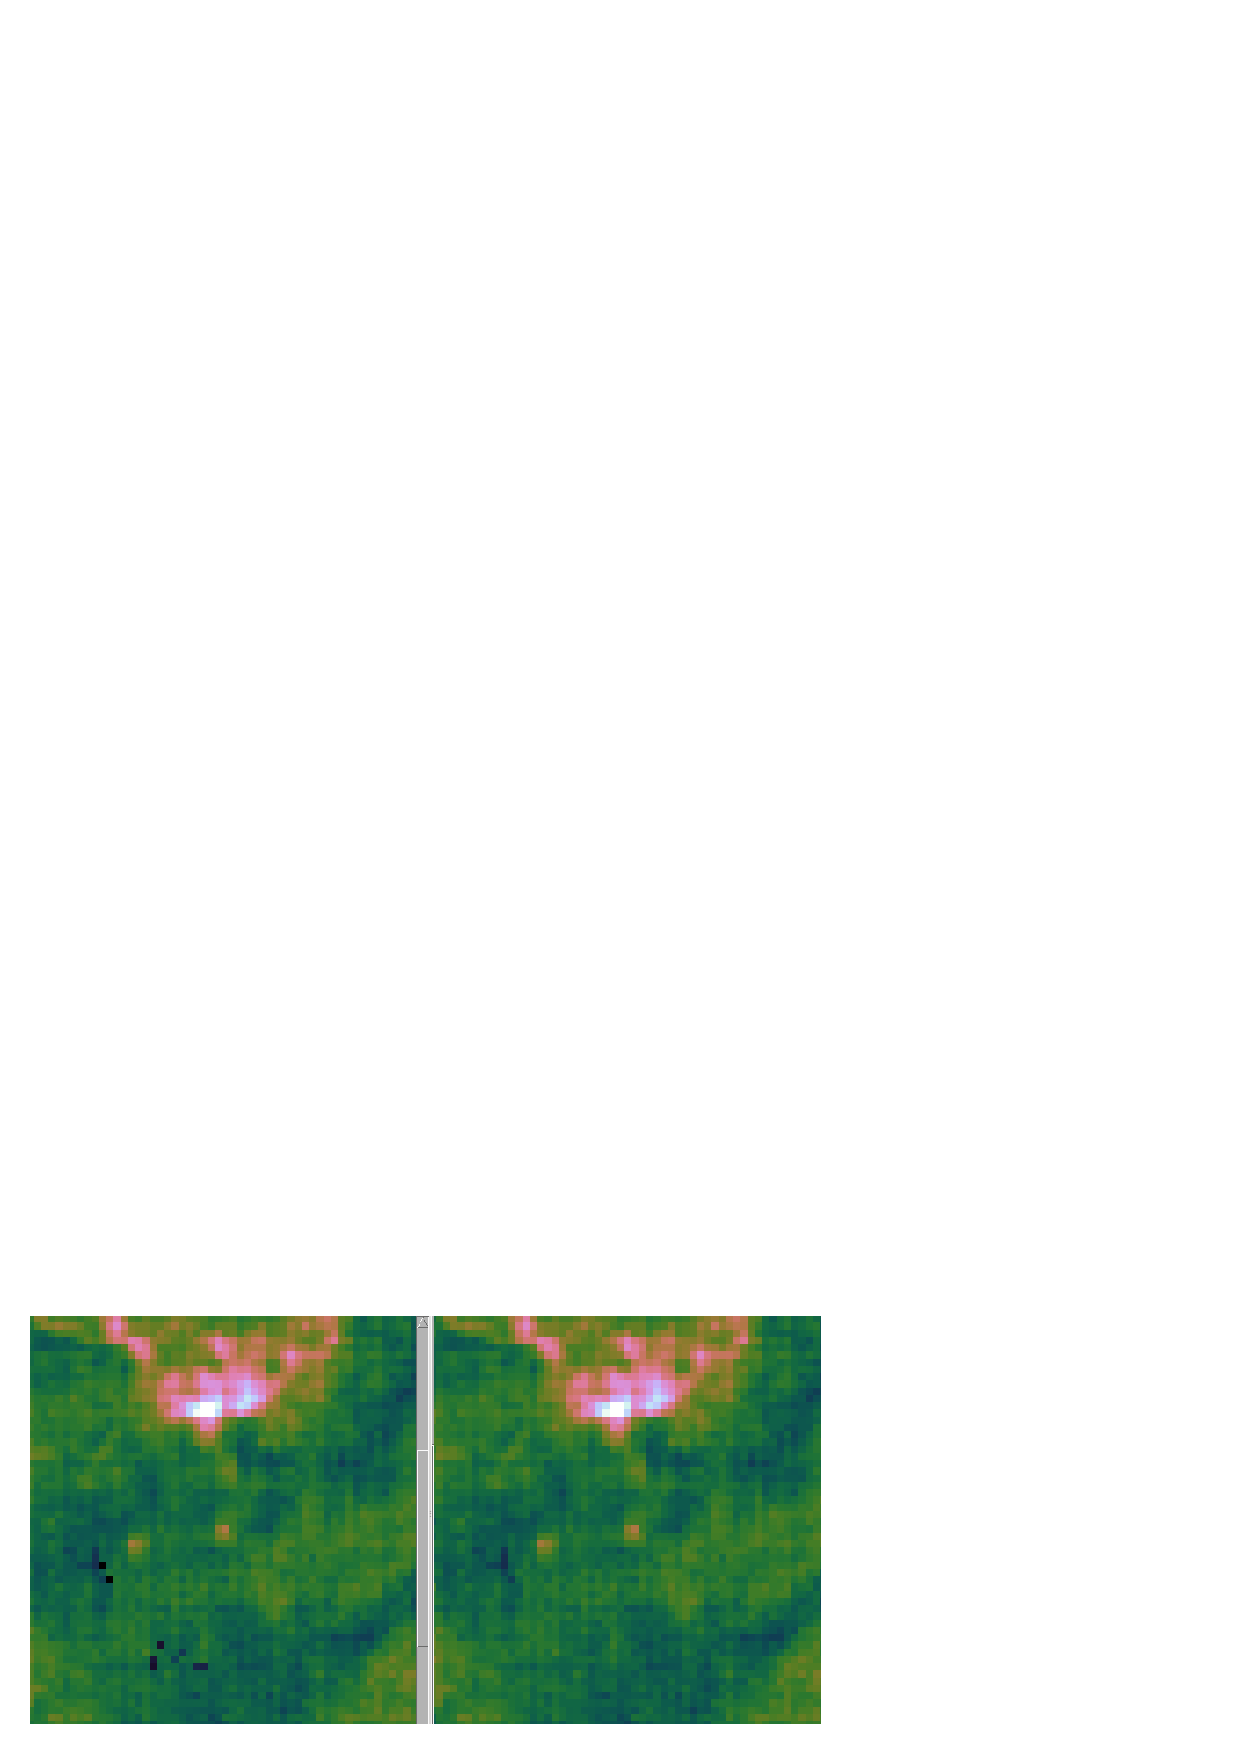
\includegraphics[width=0.8\linewidth]{sun258_fit1d_fixfit}
    \caption{Fit1d $-$  {\it Left:} Section of a parameter file showing
      originally fitted amplitudes; {\it Right:} Amplitudes after using a
      ``fixed'' parameter file from the original fit as initial estimates
      for a subsequent fit.}
    \label{fig:fixfit}
  \end{center}
\end{figure}

Another situation where manipulation of parameter files can be useful
is when parameter files from previous fits require corrections. For
instance, in case it is possible to identify the troublesome locations
with ``thresh'' those can be set to bad values and ``fillbad''
can be used to interpolate from surrounding values.

Figure \ref{fig:fixfit} shows an example. On the left is the a section
of the Amplitude plane of a parameter file resulting from a
1-component fit of a gaussian. In a few positions problems can be seen
(actually due to a secondary component).  These points were isolated
using a ``thresh'' on the Position plane of the parameters and be
interpolated over using ``fillbad''. The ``fixed'' parameter file was
then used to provide initial estimates for a subsequent file,
resulting in the fitted Amplitudes on the right.

\begin{myquote}
\begin{verbatim}
% fit1d in=infile out=outfile rms=0.22 config=^fit1d.def
% ndfcopy outfile.more.smurf_fit1d.comp_1 comp_1
% thresh comp_1'(,,2)' out=pos thrlo=2 thrhi=5 newlo=bad newhi=bad
% fillbad pos out=pos_fix
% paste comp_1 p1=pos_fix out=comp_1_fix
% fit1d in=infile out=outfile rms=0.22 config=^fit1d.def parcomp=comp_1b_fix
\end{verbatim}
\end{myquote}

These fairly simple examples are presented to illustrate the use of
``Component parameter files'', but more elaborate schemes are
possible. For instance, a section of a parameter file that fits broad
lines in the nucleus of a galaxy can be pasted into a parameter file
with narrow fits in the remainder of the disk. We'll leave further
examples to to the imagination of the reader.

\section{\xlabel{scuba2}SCUBA-2 Data Reduction\label{se:sc2dr}}

SCUBA-2 has two primary observing modes where the telescope is either
stationary relative to the source (DREAM, STARE and typically when the
FTS or polarimeter are in use), or moving (SCAN). The data processing
differs in detail for each observing mode, though the general
procedure is the same.\footnote{At the time of writing only SCAN mode
  is functional.}

In addition to data files, each observation is bracketed by dark
frames. In some cases dark frames may also be recorded part-way
through an observation. These dark frames may be used for correcting
for the drift in the bolometer zero-point and should be provided in
the list of input files for some observing modes or map-making
techniques. The iterative map-maker used for SCAN data (see
\S\ref{se:dimm}) does not require the darks and will ignore them.
 tasks that read raw data. Dark frames can be identified by searching
 for the FITS keyword \texttt{SHUTTER}, which is 0 for dark
 frames. Additionally, it is possible for short flatfield ramps to be
 taken at the start and end of an observation (see the
 \texttt{SEQ\_TYPE} FITS header) to improve the calibration. These
 files should usually be included when making maps. In general, it is
 safe to include all the files for a particular observation and leave
 it up to \SMURF\ to sort them out.

Two general approaches may be taken to reducing data. The first,
outlined by the steps in Sections \ref{se:dsworkflow} and
\ref{se:rebin}, performs all of the data reduction tasks using a range
of individual calls to \SMURF\ tasks. This method is useful if the user
wishes to interact and view each step of the reduction, although the final
maps are generally not of `science grade' quality. A second approach is to
use the Dynamic Iterative Map Maker (DIMM), described in Section
\ref{se:dimm}. All of the data pre-processing steps, as well as an
iterated solution for the final map are handled using a single
command. While the processing time may be longer, the reduced maps are
of superior quality.

\subsection{\xlabel{arraycal}Array calibration and characterization\label{se:arraycal}}

Data from array calibration observations (such as FLATFIELD and NOISE)
are processed with \SMURF. NOISE observations are used to identify
bolometers which are not in spec, from which a bad-bolometer mask can
be created. There is usually no need to re-process flatfield data
since the results have already been applied to subsequence observations, but
the techniques are included here for completeness. Both NOISE and
FLATFIELD observations can be done with the shutter closed or with the
shutter open.\footnote{Skydip observations are not available at the
  time of writing}

\subsubsection{\xlabel{flatcal}FLATFIELD\label{se:flatcal}}

FLATFIELD observations are processed with the \calcflat\ command. The
input data must be from the same observation and the same
subarray. The data are a series of frames in which the current
supplied to the internal pixel heaters is varied about a nominal value
(see the FITS keyword \texttt{PIXHEAT}). \calcflat\ solves for the
optimum heater setting given a list of resistances for each bolometer
and a reference resistor value. The list of resistances is mandatory
and requires knowledge of the subarray performance. However, a file
with suitable default values is included with the installation of
\SMURF: \texttt{\$STARLINK\_DIR/share/smurf/resist.cfg}.

The output from processing a FLATFIELD observation is a data file
(named automatically if not supplied) which contains the flatfield
solution in the NDF extension \texttt{.MORE.SCUBA2.FLATCAL}, the same
location as for the raw data. The main data array for this output file
is a three-dimensional array containing the reference-subtracted
measurements for each heater setting ($N_{\rm row}\times N_{\rm
  column} \times N_{\rm heat}$).

In addition to generating the flatfield solution, \calcflat\ can also
create a responsivity image for the current subarray. The
\aparam{RESP} parameter may be specified to store the
responsivity. The responsivity has units of amperes per watt
(A/W). Since each observation contains the flatfield, it is possible
to extract the responsibity data from any file by using the \calcresp\
command.

If for some reason this flatfield should be applied to existing data
files the \copyflat\ command can be used to copy from the file
generated by \calcflat. This is sometimes useful if a flatfield was
accepted by mistake and it needs to be corrected.

\subsubsection{NOISE}

NOISE observations are designed to check that the bolometers are
operating within specifications. This is achieved by calculating the
power spectrum and looking at the mean power between two frequencies
(usually 2 and 10 Hz). Excessively noisy bolometers are noted and a bad
bolometer mask generated.  The \calcnoise\ command can be used to
analyze any SCUBA-2 time series. It can be used to generate both a
noise image (in pA/rt(Hz)) and a NEP image (in W/rt(Hz)) from raw
data. The noise image will be the image in the main part of the data
file and the NEP image will be in the .MORE.SMURF.NEP extension. If
the data have been flatfielded the NEP image extension will not be
written since the primary image will already be in power units. A
noise ratio image (.MORE.SMURF.NOISERATIO) is also created to give an
indication of the mean power relative to the power at a particular frequency.

Bad bolometer masks are supported by the \flatfield, \extinction,
\remsky, and \makemap\ tasks through the \aparam{BBM}
parameter. A mask can be generated from the noise images using the
\KAPPA\ \thresh\ command.

\subsubsection{Comparing multiple noise or flatfield observations}

Sometimes you will find that you have many noise or responsivity
images from multiple observations and you would like to investigate the
bolometer stability. The \stackframes\ command can make this simple as
it lets you convert a directory of 2-d images into one data cube where
each frame is sorted by time. Once you have this cube you can load it
into \GAIA\ for easy visualization, use \KAPPA\ \collapse\ with
different estimators, or plot variations using \KAPPA\ \clinplot\ or \mlinplot.

\subsection{\xlabel{dsworkflow}DREAM/STARE data reduction workflow\label{se:dsworkflow}}

The DREAM/STARE observing modes (\cite{scuba2}) were originally
designed for mapping compact sources, i.e.\ those which are smaller
than the field of view of SCUBA-2 (approximately 8 arcmin). Although
these modes have not been commissioned at the time of writing and it
is thought that STARE mode will not work, it is nevertheless more
straightforward to discuss DREAM and STARE first.

The workflow for processing DREAM and STARE data may proceed in one of
two ways: a simplified workflow using images calculated by the data
acquisition (DA) at the time of the observation, or the full workflow
starting from the raw data. The full procedure is described below, and
steps which are unnecessary in the simplified workflow are noted.

The workflow proceeds as follows:
\begin{enumerate}
\item Apply flatfield solution (full only);
\item Remove atmospheric emission;
\item Correct for atmospheric extinction;
\item Calculate images from time-series (full only);
\item Combine images to create output mosaic.
\end{enumerate}

\subsubsection{DA images}

The images calculated by the DA are stored as NDF extensions in the
raw data files under \texttt{.MORE.SCU2RED.In} where \texttt{n} is an
integer (non-zero-padded). Each image is an average of the data in
typically 1 second. Note the final image is created from whatever
samples remain if the duration of the file is not an integer number of
seconds. Each image has its own FITS header associated with it which
contains values which vary between images.

\subsubsection{\xlabel{flatfield}Applying the flatfield correction\label{se:flatfield}}

This section describes how to apply the flatfield solution to raw
data. This step is not necessary for the simplified workflow.

A FLATFIELD observation records variation in the sensitivity of each
bolometer. Ideally, every bolometer gives the same reading when
exposed to a calibrated radiation source. In practice, each one
responds in a slightly different way.

The flatfield response for each subarray is derived at the telescope
from a dedicated FLATFIELD observation. This solution is written to
all subsequent data files until a new solution is derived (see Section
\ref{se:flatcal} above).

Bolometer output is modified by the gain of the individual bolometer
and its offset from a one-to-one relationship with the input
radiation. Thus the output power from bolometer $i$ is related to the
input (optical) power by:
\begin{equation}
P_{{\rm out},i} = G_i P_{{\rm in},i} + O_i.
\end{equation}
where $G$ is the gain and $O$ is the offset.

The \SMURF\ routine that applies the flatfield correction is called
\flatfield. Since the flatfield information is already included in
each subscan, multiple files can be flatfielded with a single call to
the \flatfield\ routine; there is no need to process files from
different subarrays separately. Dark frames should be included in the
list of input files in order to correct for bolometer zero-point
drifts. Note that only flatfielded data (non-dark) files are written
out, and that the naming scheme will change. The list of output files
given is truncated at the appropriate number. The list of files
actually written to disk is obtained via the \aparam{OUTFILES}
parameter if specified.

\subsubsection{\xlabel{skysub}Removing the atmosphere\label{se:skysub}}

This section describes how to subtract the signal from the atmosphere
(or sky) from your observations. This step is required for both the
full and simplified workflows.

The sky is highly emissive (bright) at submillimetre
wavelengths\cite{archibald}, and the radiation received from an
astronomical source is only a very small fraction of the radiation
received from the atmosphere. Typically the atmospheric signal is a
factor of $10^5$ times greater than that from the source (see Figure
\ref{fig:signal} for a pictorial representation). In addition, the
atmospheric emission varies significantly over the timescales of a
typical observation, further swamping any contribution from the
source. Fortunately, the emission from the sky is correlated over the
SCUBA-2 field of view, which enables simple sky removal techniques to
be used effectively\cite{archibald,sc2ana002}.

\begin{figure}[htb]
  \begin{center}
    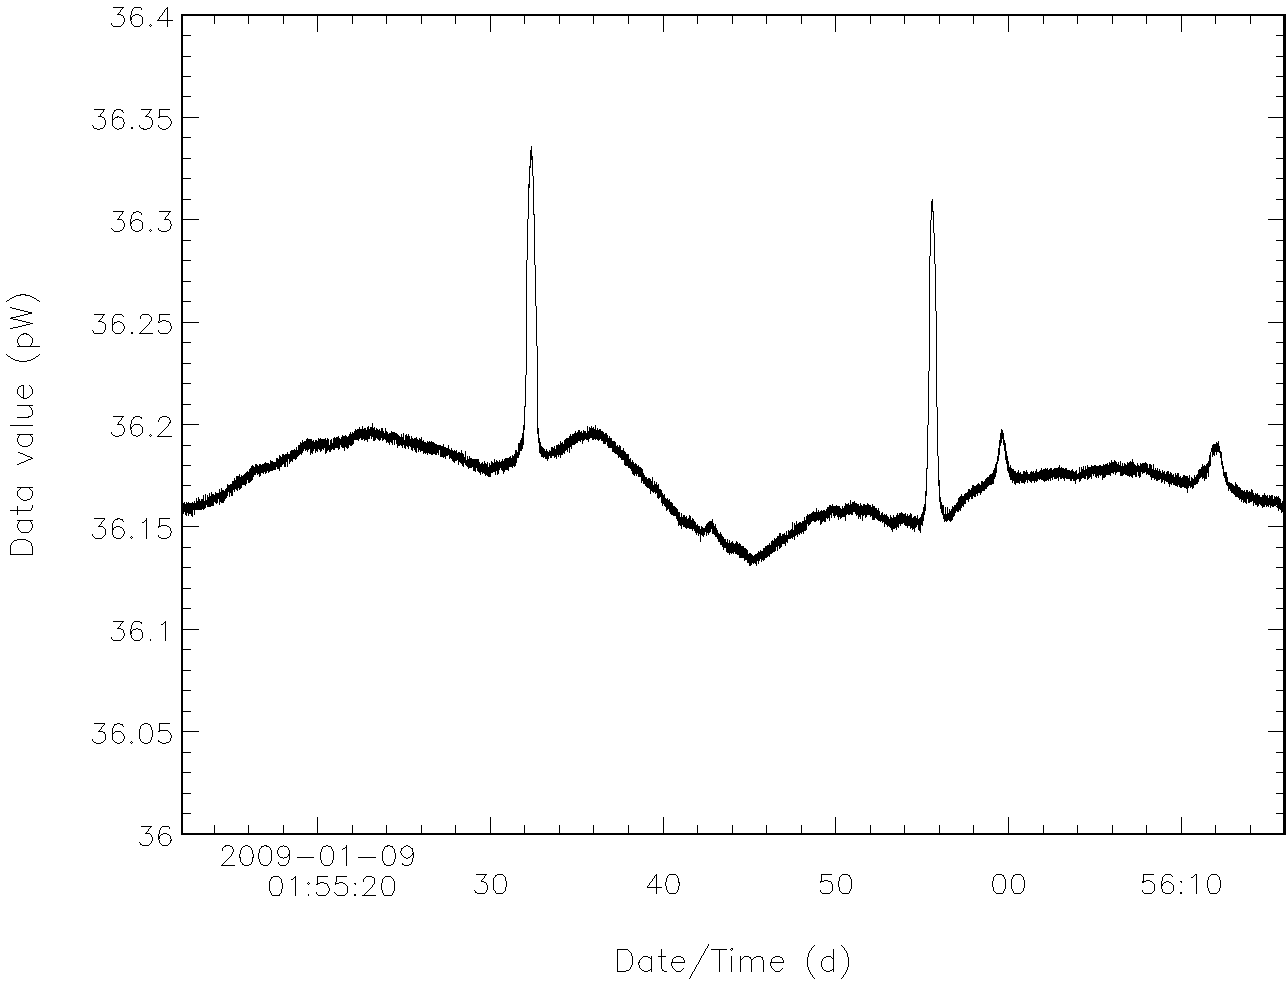
\includegraphics[width=150mm]{sun258_submmsignal}
    \caption{Illustration of the relative magnitudes of atmospheric
      and source signals at submillimetre wavelengths. Data are from
      850 $\mu$m observations of Jupiter with SCUBA-2. The sharp
      features occur when Jupiter is seen by the bolometer. The
      increase in optical power from Jupiter is $\sim$0.5\%. Most
      sources will be many thousands of times fainter.}
    \label{fig:signal}
  \end{center}
\end{figure}

In a single sample the signal collected from an astronomical source is
negligible in comparison with the contribution from the
atmosphere. Many samples are required to collect a statistically
significant signal from the source.

The \SMURF\ routine that removes the sky is called \remsky\ and has
several options for fitting and removing the atmospheric contribution
to the signal. All take advantage of the fact that the sky signal is
correlated between adjacent bolometers.

The atmospheric signal can be fit in the following ways:
\begin{itemize}
\item Calculate the mean value of the signal;
\item Fit a gradient in elevation only;
\item Fit a plane of arbitrary orientation.
\end{itemize}
Furthermore, \remsky\ can make use of the data from all available
subarrays simultaneously to make a better estimate of the atmospheric
emission (see the \aparam{GROUP} parameter).

For simple cases, subtracting a mean value may be sufficient, though
it is not recommended for bright sources, as the mean will be biassed
too high by the presence of the source. A more sophisticated solution
may be obtained by fitting a plane to the data. The plane may have
arbitrary orientation (in azimuth and elevation) or may be fixed so
that the slope is in elevation only.

\subsubsection{\xlabel{extinction}Correcting for atmospheric extinction\label{se:extinction}}

This section describes how to correct your data for atmospheric
extinction, the loss of radiation from the source as it travels
through the atmosphere. This step is required for both the full and
simplified workflows.

The observed signal from an astronomical source decreases as the
atmosphere along the line of sight increases. At lower elevations,
there is more atmosphere along the line of sight between the source
and the telescope.

The radiation received by SCUBA-2 is the sum of the radiation from the
astronomical source (represented by $I_{\rm src}$ in Equation
\ref{eq:iobs} below) and the radiation from the atmosphere ($I_{\rm
  atm}$). However, $I_{\rm src}$ is diminished by the optical depth
of the atmosphere ($\tau$) as follows:
\begin{equation}
I_{\rm obs} = I_{\rm atm} + I_{\rm src} \exp(-\tau).
\label{eq:iobs}
\end{equation}
The optical depth is usually quoted as the value at the zenith
($\tau_{\rm zenith}$), but you need the value of tau at the same
elevation as your observations ($\tau_{\rm obs}$). For a
plane-parallel atmosphere, $\tau_{\rm obs} = A \times \tau_{\rm
  zenith}$, where airmass ($A$) is a measure of the total atmosphere
along the line of sight.

Airmass is defined as $1 / \cos \theta$, where $\theta$ is the zenith
angle. The zenith angle is the vertical angle measured from the zenith
($\theta = 0^\circ$) towards the horizon ($\theta = 90^\circ$) and is
thus equal to $90-\phi$, where $\phi$ is the elevation. You can now
calculate $\tau_{\rm obs}$ from $\tau_{\rm zenith}$ and $\phi$ as
follows:
\begin{equation}
\tau_{\rm obs} = \tau_{\rm zenith} / \cos(90^\circ - \phi ).
\label{eq:tau}
\end{equation}

Using Equation \ref{eq:tau}, rewrite Equation \ref{eq:iobs} as:
\begin{equation}
I_{\rm obs} = I_{\rm atm} + I_{\rm src} \exp \left(
\frac{-\tau_{\rm zenith}}{\cos(90^\circ-\phi)}\right).
\end{equation}
%The top graph in Figure ??? shows how the observed signal varies with elevation
%and airmass.

The elevation angle of each bolometer can be calculated, and given
$\tau_{\rm zenith}$ \remsky\ calculates the $\tau_{\rm obs}$ at the
elevation angle of each bolometer.

The zenith optical depth can be obtained via three methods:
\begin{enumerate}
\item Skydips: The zenith optical depth is derived from a SKYDIP
  observation, in which the signal at each wavelength is recorded over
  a range of airmasses. \SMURF\ does not yet have the capability to
  process SCUBA-2 skydips.

\item CSO tipping radiometer: The Caltech Submillimeter Observatory
  (CSO) radiometer measures $\tau_{\rm zenith}$ from skydip
  observations at 225 GHz. The CSO radiometer records a new $\tau_{\rm
    zenith}$ every 10 minutes and values are stored in the FITS
  headers corresponding to the start and end timestamps of the file
  (\texttt{TAU225ST} and \texttt{TAU225EN}). \SMURF\ converts CSO
  $\tau_{\rm zenith}$ to $\tau_{\rm zenith}$ at 450 or 850 $\mu$m,
  relying on an empirical relationship between $\tau_{\rm zenith}$ at
  225 GHz and $\tau_{\rm zenith}$ at 450 or 850 $\mu$m.

\item JCMT Water Vapour Monitor: The JCMT Water Vapour Monitor (WVM)
  provides opacity estimates every 1.2 seconds by measuring the
  spectral shape of the 183 GHz water line along the telescope
  line-of-sight, and then converting this to an effective $\tau_{\rm
    zenith}$ at 225 GHz. Since the measurement is aligned with the
  submillimetre beam this method circumvents the need to apply the
  plane parallel approximation (which breaks down at the horizon). The
  raw WVM data are stored in the JCMT state structure, though the
  values at times corresponding to the start and end of the file are
  stored in the FITS headers (\texttt{WVMTAUST} and
  \texttt{WVMTAUEN}).
\end{enumerate}
Optical depth measurements derived from the WVM are most useful in
variable atmospheric conditions where the CSO radiometer may not be
giving sufficiently-frequent readings.

The \SMURF\ routine that corrects for atmospheric extinction is called
\extinction. The \extinction\ routine can use $\tau_{\rm zenith}$
determined by all of the above methods, and obtains values
automatically from the FITS headers for the WVM and CSO cases or uses
the raw WVM data if desired.

The user can choose how accurate a correction they wish to apply using
the \aparam{METHOD} parameter. By default, \extinction\ will assess
the magnitude of the correction and if it does not change
significantly across the field of view, then a single value is used
(corresponding to the elevation of the tracking position). If there is
a significant variation, then \extinction\ will apply a correction to
each bolometer using the elevation of that bolometer. It is possible
to enforce either of these options by setting \aparam{METHOD} to
\texttt{QUICK} or \texttt{FULL} respectively.

Note that sky subtraction must take place before the extinction
correction is applied. \extinction\ checks the history to see if
\remsky\ has been run and exits with an error if not. However, if an
alternative method of sky subtraction has been used (such as using
\KAPPA\ \csub\ to subtract a mean or median value) then the
\aparam{HASSKYREM} may be set to \texttt{TRUE} to override the history
check by \extinction.

\subsubsection{\xlabel{dsimages}Calculating images from time-series
  data\label{se:dsimages}}

This step is not required for the simplified workflow.

\SMURF\ provides separate routines for calculating images from STARE
and DREAM data. STARE images are calculated with \starecalc; DREAM
images are calculated with \dreamsolve.

In \starecalc\ the user may specify how many samples to average to
create images (the default is to calculate averages once a second).

\dreamsolve\ requires the DREAM weights file specified in the FITS
header keyword \texttt{DRMWGHTS} to reside in the current
directory. Data from each subarray require a corresponding weights
file. See section \ref{se:dream} below for details on calculating
alternative weights files.

\subsubsection{\xlabel{mosaic}Combining the images\label{se:mosaic}}

\SMURF\ does not have any image mosaicking tasks itself. This step is
handled by routines in \KAPPA\ and \CCDPACK. Suitable tasks are
\wcsmosaic\ in \KAPPA\ and a combination of \KAPPA\ \wcsalign\ (to
align all the images to a common coordinate frame) followed by
\CCDPACK\ \makemos.

See the SMURF cookbook (\SMURFcook) for more detailed information
about mosaicking SCUBA-2 images.

\subsubsection{\xlabel{dream}Using alternative DREAM solutions\label{se:dream}}

This step is not usually necessary for either workflow but is included
for completeness.

The DREAM observing mode moves the secondary mirror in a pattern which
causes adjacent bolometers to observe the same region of the sky
multiple times \cite{scuba2,dream}. The data are then described by a
series of simultaneous equations which are solved via a matrix
inversion (using singular value decomposition). Since the pattern
traced out by the secondary mirror is known, the inverse of the matrix
can be pre-calculated (a time-consuming task) for a given output grid
and applied to data at the time of observation (quick).

It is {\em strongly} recommended that users become familiar with the
details of DREAM \cite{dream} before using weights other than the
default for science data processing.

The user may wish to experiment with different regridding schemes or
there may be other reasons, not known at the time of observation,
which require the inverse matrix to be re-calculated. The task for
doing this is called \dreamweights, and this allows the user to
specify different output grid parameters. The calculation of the
inverse is moderately time-consuming (compared with calculating the
images) and takes of order 5--10 minutes on current hardware. The
output file from \dreamweights\ is the weights file required by
\dreamsolve. \KAPPA\ \fitsedit\ may be used to specify weights files
which differ in name from the default. Note that this process must be
repeated for each subarray for which data exist and that data which
are to be combined should all use the same grid.

\subsection{\xlabel{scanworkflow}SCAN data reduction
  workflow\label{se:scanworkflow}}

Processing SCAN data is more complicated than DREAM and STARE data.
The challenge is to make an image when the data taken at each
bolometer position do not line up exactly with the output map
pixels. The fundamental difference is that the primary mirror is
scanning the array continuously on the sky. The pixels in the map can
therefore be chosen arbitrarily, and bear no relationship with the
array of detectors \cite{sc2ana001,sc2ana005,sc2ana006}.

\SMURF\ supports two methods of creating a map:
\begin{enumerate}
\item A simple rebinning algorithm to assign data to output map
  pixels, sometimes referred to as a `naive map';
\item An iterative method which solves for a succession of model
  components assumed to represent the raw data.
\end{enumerate}

The rebinning method may be adequate for bright compact sources
(bright enough to be detected in one sample and smaller than the field
of view of the array). The rebin method is also suitable for obtaining
a `quick-look' image and vital when you wish to make maps of some of
the models generated by the iterative map-maker. The \SMURF\ task
\makemap\ supports this map-making method.

In practice, the dynamic iterative map maker (DIMM; see Section
\ref{se:dimm}) will generally give superior results, though it is more
computationally intensive. \makemap\ supports the DIMM.

\subsubsection{\xlabel{rebin}Rebinning map-maker\label{se:rebin}}

The processing of SCAN data with the rebin method proceeds in a
multi-step approach that follows the method listed above for DREAM and
STARE data using \makemap. A one-pass rebinning algorithm is applied
to the data, which regrids the signal from each bolometer on to a map
in the desired co-ordinate system.

As outlined in \ref{se:dsworkflow}, the procedure for processing
SCUBA-2 data follows these steps:
\begin{enumerate}
\item Apply the flatfield correction (see Section \ref{se:flatfield});
\item Clean the data set using \clean. This can remove spikes, DC
  steps and low- and high-frequency components in the data.
\item Remove the contribution of atmosphere to the signal (see Section
  \ref{se:skysub});
\item Correct for atmospheric extinction (see Section
  \ref{se:extinction});
\item Make a map using the rebin method.
\end{enumerate}

The rebinning algorithm shares the observed signal from a single
bolometer between neighbouring output map pixels, as determined by the
pixel-spreading function. The value of each pixel in the map is the
sum of the signal from every bolometer that observed at that position.

There are many options for the pixel spreading scheme (see the \wcsmosaic\
documentation for a summary). The fastest option is to use the nearest-neighbour
pixel spreading scheme (`Nearest'), which assigns the whole signal
from one bolometer to the nearest map pixel. This option does not
always produce smooth maps (if the map is poorly sampled, for example,
but it produces a robust estimate of the noise. In the limit of a
large number of `hits' per pixel, and with a pixel size sufficiently
small compared to the beamsize, this method is optimal.

For smoother maps (with poor sampling, for example), the `Linear'
scheme can be used to share the input signal equally among the four
nearest map pixels. There are more complicated options available,
e.g., Sinc-type functions, or Gaussian distributions. These methods
produce aesthetically pleasing maps, at the risk of introducing
correlations into the noise and additional smoothing to the map.

Figure \ref{fig:rebinmap} shows an example map created from simulated
observations of an extended source with bright features. It was
created using the rebin method and the nearest-neighbour pixel
spreading scheme.

Note the dark regions around the bright sources. They are negative
bowls introduced by the sky subtraction method (Section
\ref{se:skysub}). The random dots are cosmic ray spikes which are not
removed by this particular workflow.

\begin{figure}[htb]
  \begin{center}
    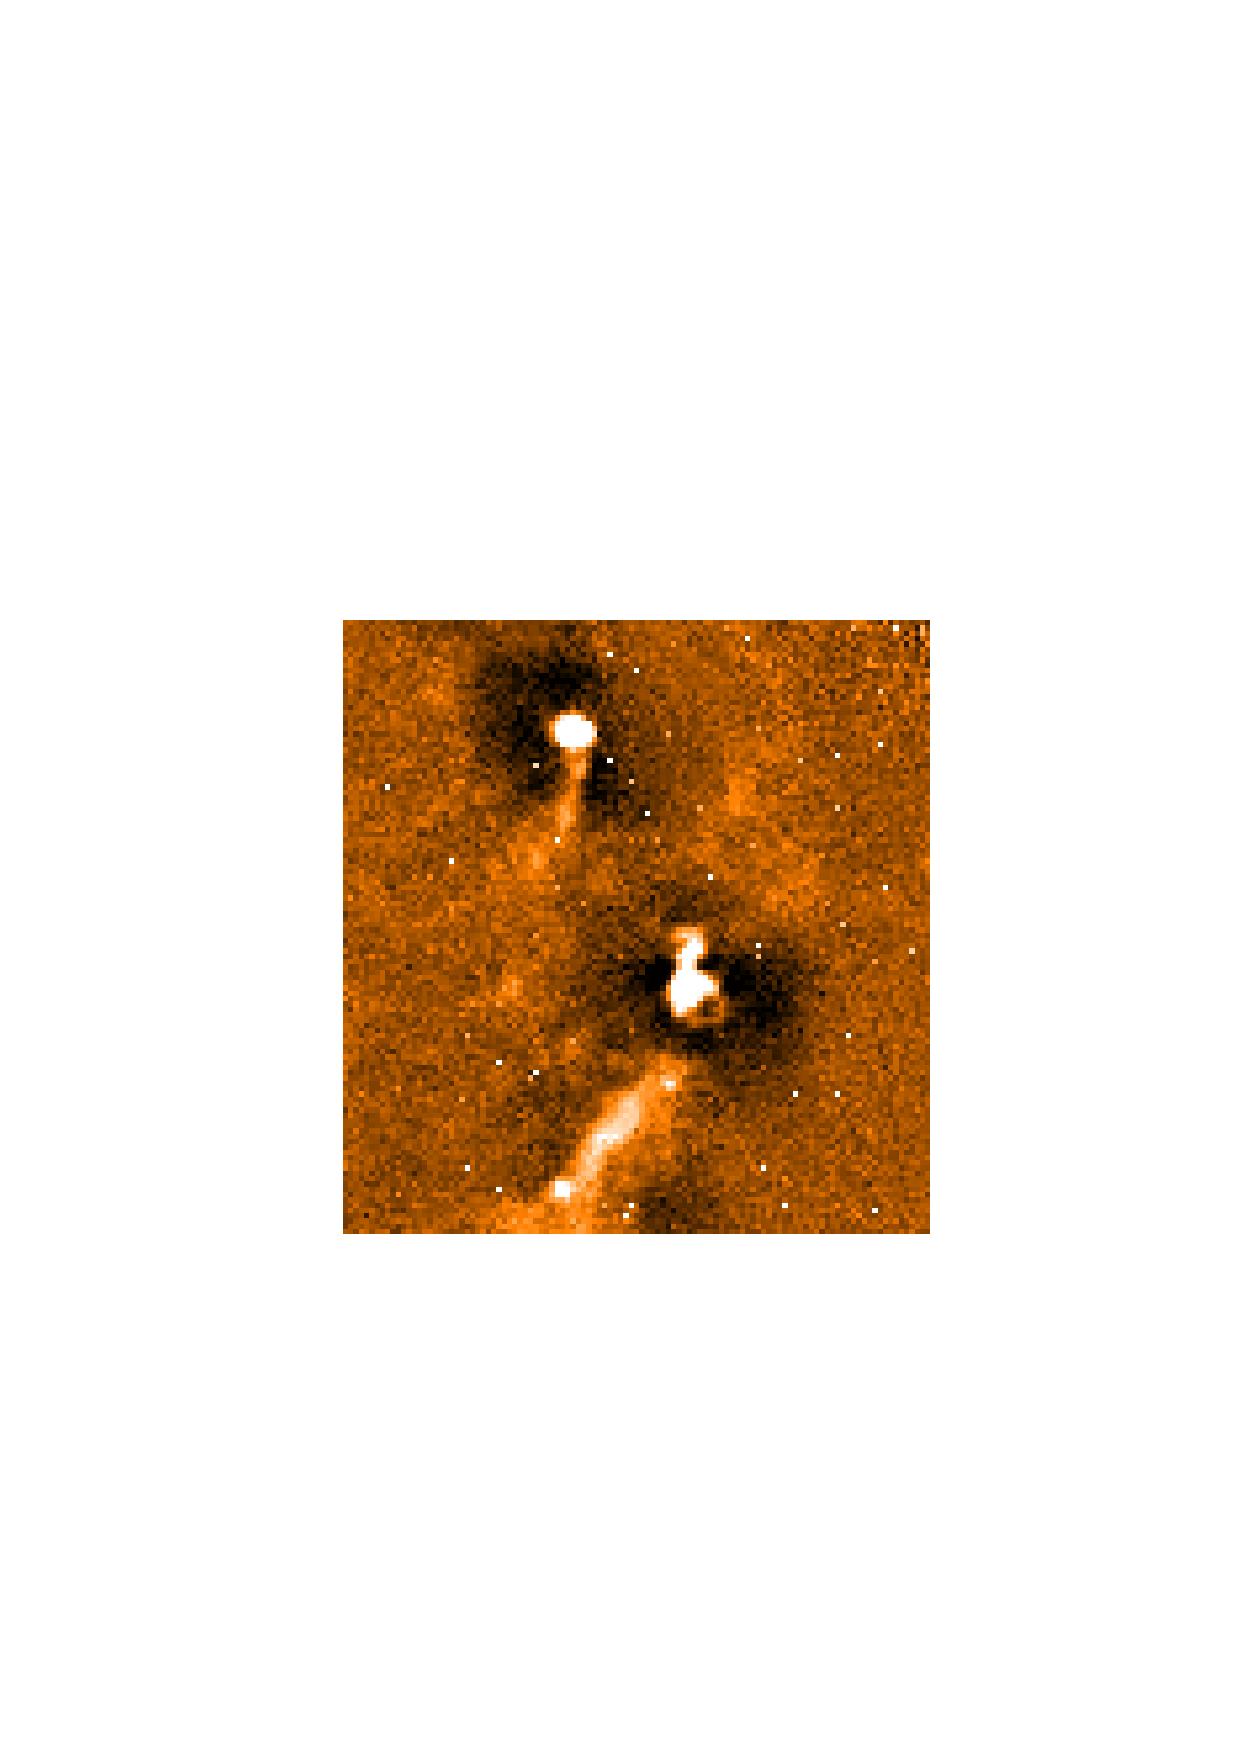
\includegraphics[width=0.7\linewidth]{sun258_rebinmap}
    \caption{Image reconstructed from simulated data using the
      \aparam{REBIN} method. Note the deep wells around bright
      sources and the numerous spikes caused by (simulated) cosmic
      rays.}
    \label{fig:rebinmap}
  \end{center}
\end{figure}

\section{\xlabel{dimm}SCUBA-2 Dynamic Iterative Map-Maker\label{se:dimm}}

The Dynamic Iterative Map-Maker (DIMM) is the preferred tool for
producing maps of SCUBA-2 total power data obtained in SCAN
mode\cite{sc2ana006} (see also \SMURFcook). Rather than executing each
of the steps described in Section \ref{se:rebin} separately, the DIMM
is capable of performing all of the data pre-processing steps, as well
as iteratively solving for multiple signal components (including the
image of the astronomical sky) using a single call to the \makemap\
task.

\subsection{Signal model}

We first develop the model used by the DIMM for time-varying bolometer
signals as a linear combination of several components:
%
\begin{equation}
I^i_{\mathrm{obs}}(t) = [G_C^i COM(t) + O_C^i] + [G_D^i DKS^j(t) + O_D^i] +
                      EXT^i(t) AST^i(t) + N^i(t).
\end{equation}
%
Here $I^i_{\mathrm{obs}}(t)$ is the total power delivered to the $i$th
detector in pW as a function of time. The actual data written to disk
have some arbitrary digital units that are proportional to pW. The
conversion to pW is accomplished by flatfield measurements described
in Section \ref{se:flatcal}. Figure \ref{fig:comps} shows a pictorial
representation of some of the components, and they are also described
in Table~\ref{tab:dimm_components}.

\begin{table}
\begin{tabular}{cp{10cm}}
 Model Component & Definition \\
\hline
$COM$ & Removes common-mode signal, i.e., the signal seen by all bolometers. This removes most of the atmospheric emission. In addition bad detectors are also flagged if there signal does not resemble the common mode measured by the other detectors. \\
$GAI$ & If $COM$ specified, a gain and offset is used to fit $COM$ to each detector before removal. \\
$DKS$ & Fits gain and offset to remove signal recorded by dark SQUIDs. \\
$EXT$ & Applies the extinction correction. \\
$AST$ & Triggers map estimation, and removal of astronomical signal from the time-series. \\
$FLT$ & Applies a frequency domain filter. \\
$SMO$ & Smooths by using a mean or median in a moving window. \\
$PLN$ & Fit a 2d plane to each time slice. \\
$TMP$ & Use a JCMTSTATE template as a model. \\
$NOI$ & Estimates the time-domain variance to establish relative detector weights for the map estimated, and for chi-squared ($\chi^2$) tolerance. \\
\hline
\end{tabular}
\caption{Model Components for Iterative Mapmaking}
\label{tab:dimm_components}
\end{table}

\begin{figure}[htb]
  \begin{center}
    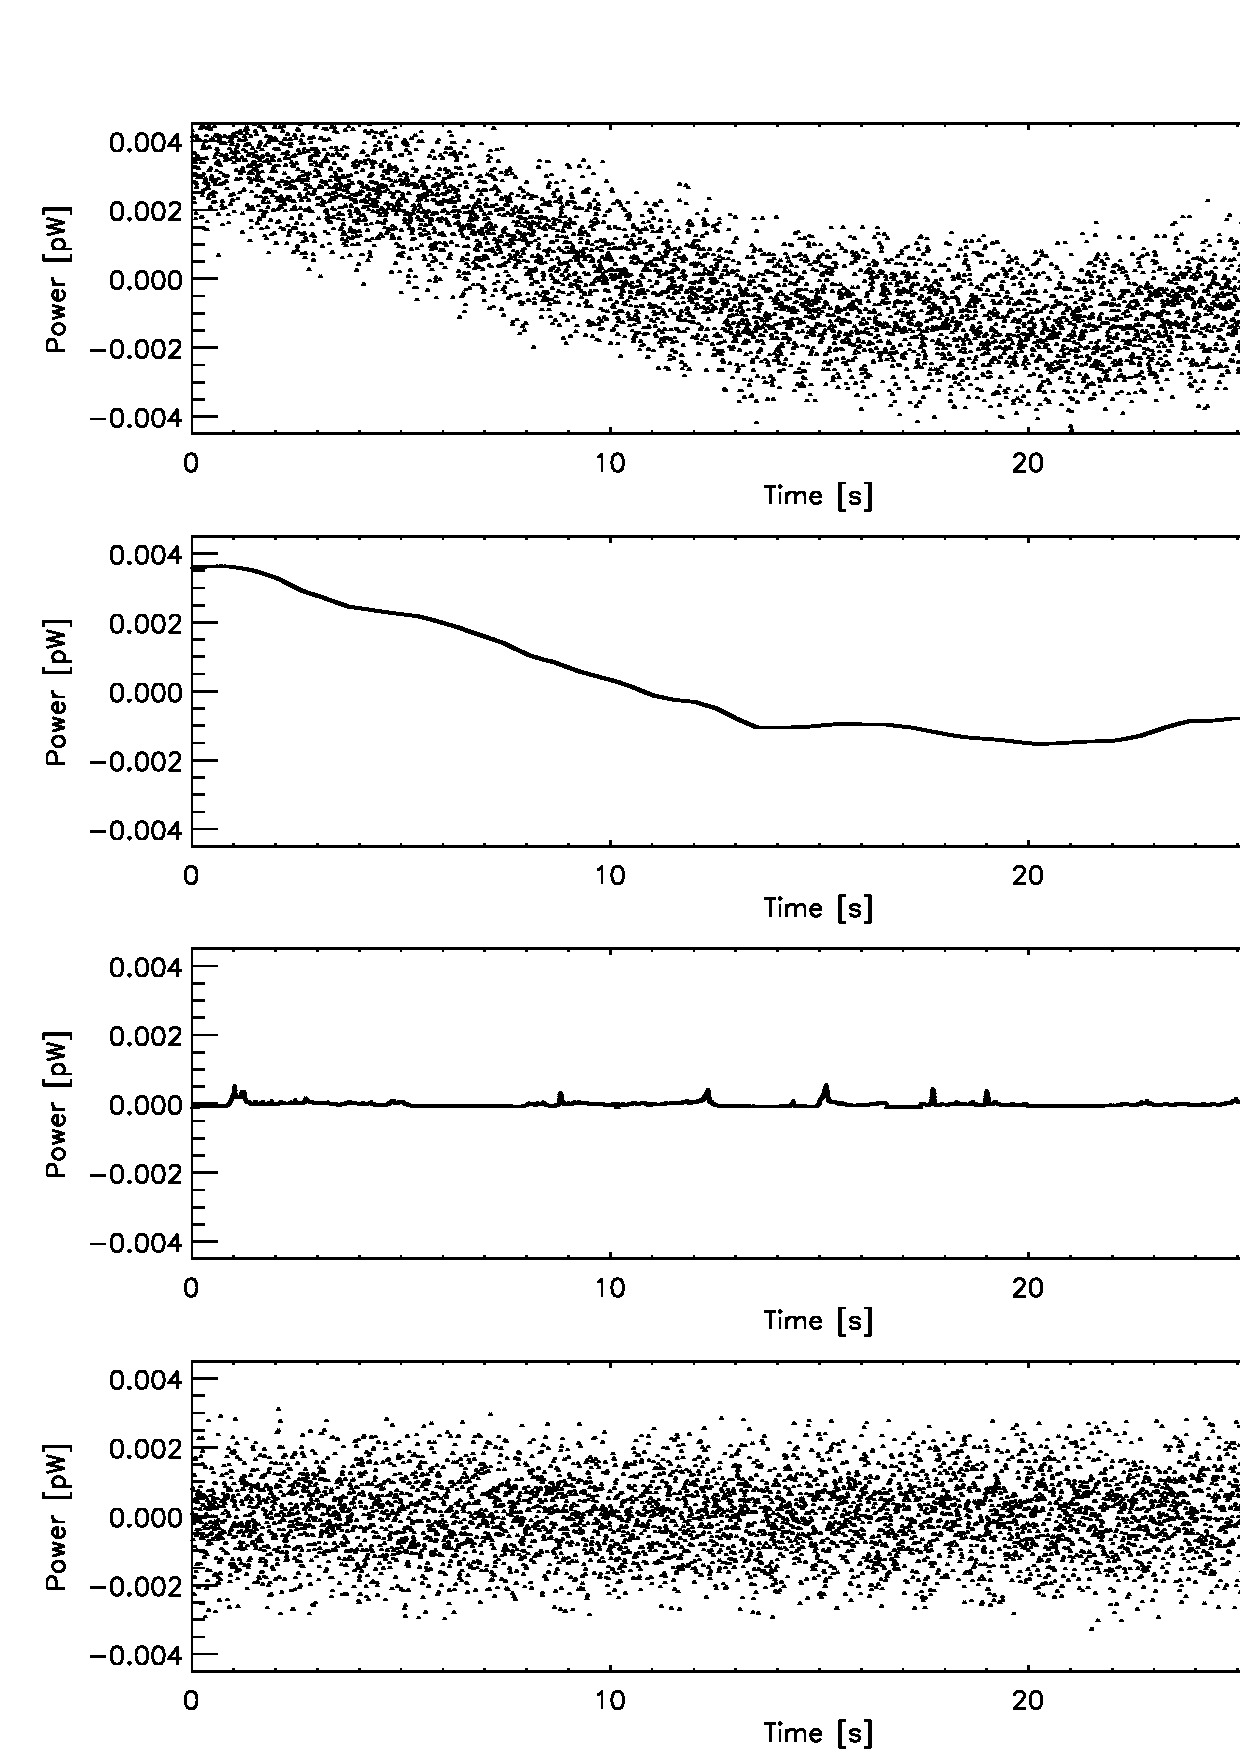
\includegraphics[width=0.76\linewidth]{sun258_signalcpts}
    \caption{Simulation of bolometer time-series showing some of the
      components that make up the total signal. The top panel shows
      the observed signal, with subsequent panels showing the relative
      contributions from the atmosphere, the astronomical source and
      white noise.}
    \label{fig:comps}
  \end{center}
\end{figure}

There is a dominant signal seen almost equally by all of the
detectors. This `common-mode' component, $COM$, is a mixture of
emission from atmospheric water vapour and the ambient thermal load
from the telescope itself. Each detector has two free parameters
associated with this signal component: a gain, $G_C^i$, and offset,
$O_C^i$. This enables the map-maker to handle cases where the
flatfield has a small residual error, and/or small residual baseline
offsets are present.

The first successful observations with SCUBA-2 used test arrays that
exhibited strong signals correlated along columns (believed to be
caused by magnetic field pick-up). Dark SQUIDs, $DKS$, (readouts with
no thermal absorbers) at the ends of
%the $j$th
each
column seem to provide
a good measurement of this signal. Similar to $COM$, the DIMM can fit
a gain and offset, $G_D^i$ and $O_D^i$, to each detector for the
appropriate dark SQUID signal in the $j$th column.

The actual astronomical signal from which we wish to make a map,
$AST$, is attenuated by an extinction factor, $EXT$, resulting from
absorption by atmospheric water vapour. The calculation of $EXT$ is
described in detail in Section \ref{se:extinction}. The ultimate goal
of the DIMM is to isolate the component of the bolometer signals
produce by $AST$ and to re-grid it into a map.

Finally, there is a residual noise term for each detector, $N^i(t)$,
which includes all of the remaining signal not accounted for by the
other model components. Ideally the dominant part of this signal would
be the white noise resulting from the thermal background, the noise
component responsible for the noise equivalent power (NEP) and
corresponding noise equivalent flux density (NEFD) used to plan
observations. In practice, the detectors also have other
slowly-varying baselines that are independent of the correlated $COM$
and $DKS$ signals described above. Therefore we express the residual
noise as
%
\begin{equation}
N^i(t) = N^i_{\rm w}(t) + N^i_{\rm lf}(t),
\label{eq:dimm_noise}
\end{equation}
%
where $N^i_{\rm w}(t)$ and $N^i_{\rm lf}(t)$ are the white and
independent low-frequency noise components, respectively. The DIMM can
attempt to fit $N^i_{\rm lf}(t)$ using the $FLT$ model component such
that the residual signal is given only by $N^i_{\rm w}(t)$.

The strategy used by the DIMM is to estimate each of the signal
components sequentially, roughly in order of decreasing amplitude. At
the end of this procedure a numerical value proportional to $\chi^2$
(quantifying the mismatch between the model and the data) is
calculated from the r.m.s. in the residual noise $N^i_{\rm
  w}(t)$. Provided that the model components are in some sense
`orthogonal', multiple iterations of this procedure produces improved
estimates of each component with stable convergence properties. This
can be checked by monitoring the value of $\chi^2$: if the change
between subsequent iterations is small enough the DIMM can stop
automatically. Alternatively, a set number of iterations may be
requested. In the future, separate convergence tests for each model
component may be added.

\subsection{Detailed operation\label{se:dimmdetails}}

\begin{figure}
\begin{center}
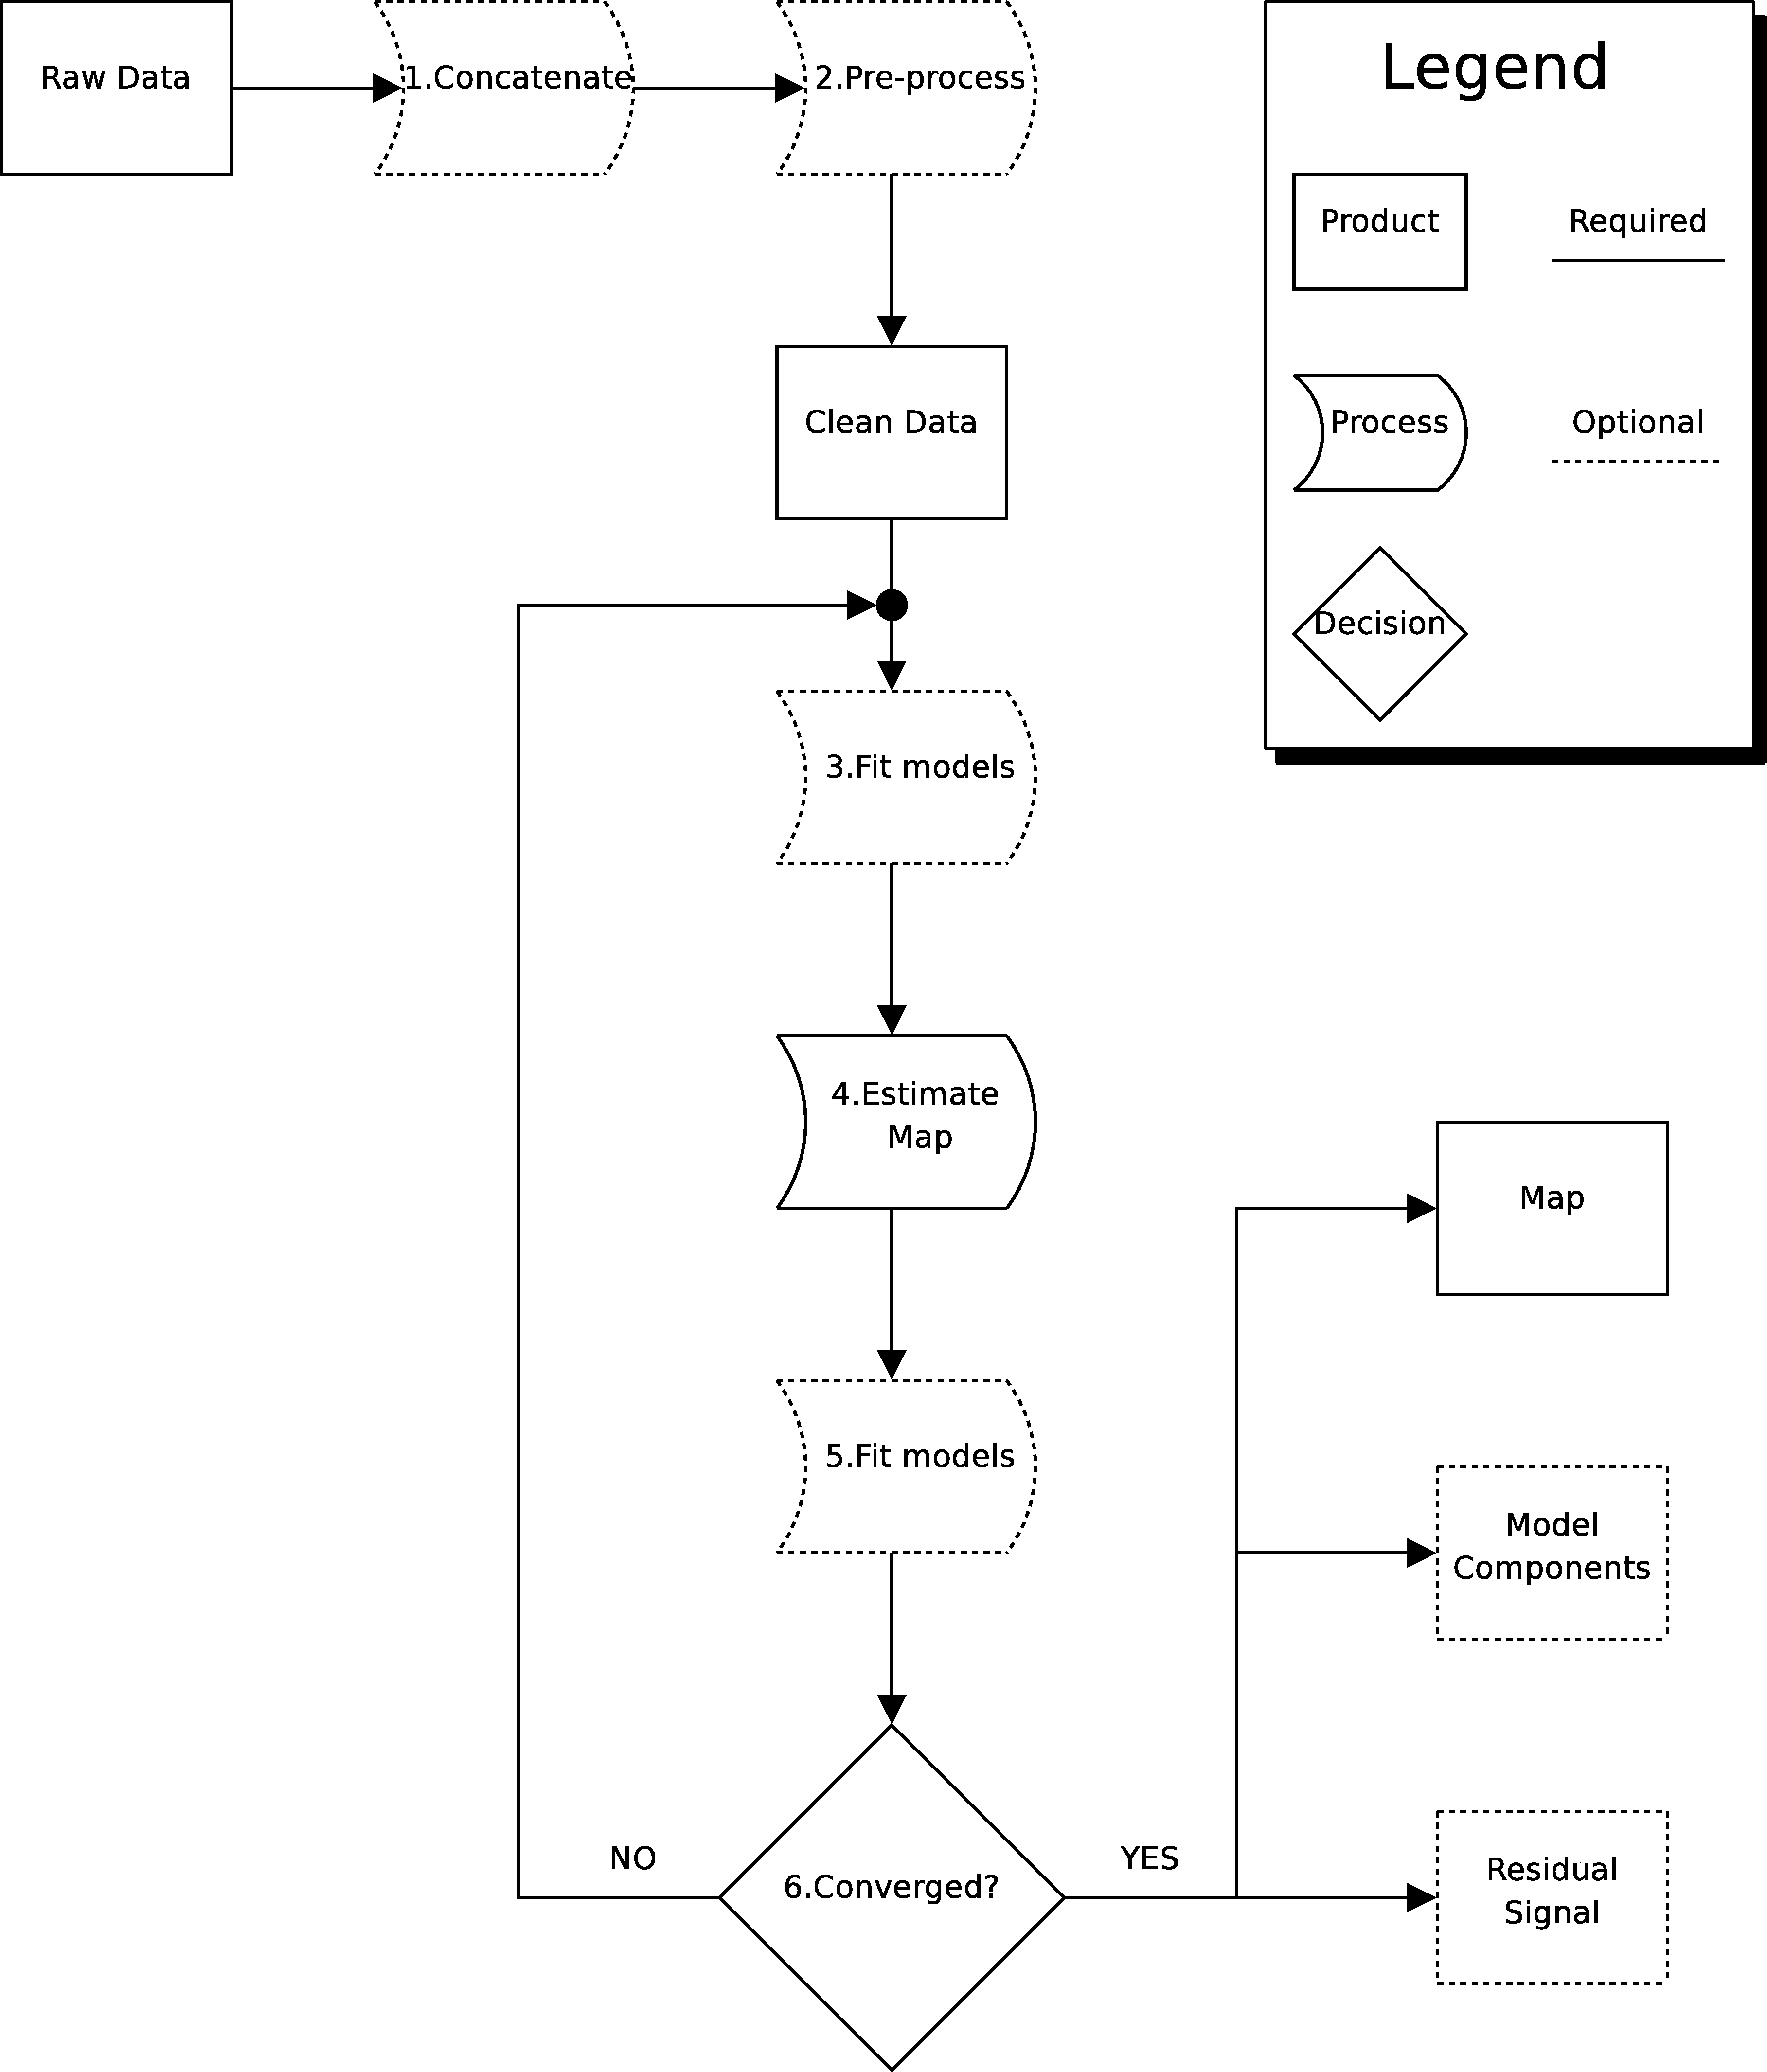
\includegraphics[width=\linewidth]{sun258_dimm_flow}
\caption{Flow chart depicting operation of the dynamic iterative
  map-maker (DIMM).}
\label{fig:dimm_flow}
\end{center}
\end{figure}

Most of the processing steps followed by the DIMM are controlled by a
configuration file (see configuration file parameters for the
\makemap\ task). An overview of the DIMM operation is shown in
Figure~\ref{fig:dimm_flow}, and the numbered boxes are described
below:

\begin{description}

\item[1. Concatenate:] The \makemap\ task typically takes raw SCUBA-2
  data as its input. The best maps are produced by first concatenating
  as much data from a given observation as possible into single
  continuous data streams in memory. This step is controlled by the
  \cparam{MAXLEN} configuration file parameter, as well as the \makemap\
  parameter \aparam{MAXMEM}. When the files are concatenated, it is
  also possible to add extra padding at the beginning and end of the
  data streams to facilitate filtering (see the \cparam{PAD} and
  \cparam{ZEROPAD} configuration file parameters). This operation is
  equivalent to using the \concat\ task.

  Whether concatenation is requested or not, it is also worth noting
  that \makemap\ automatically applies the internally stored flatfield
  as data files are loaded, so that they have units of pW before
  estimating the map.

\item[2. Pre-process:] Before the iterative process begins, several
  pre-processing (data cleaning) steps may be applied. See the
  configuration file parameters \cparam{APOD, ORDER, BADFRAC,
    FLAGSTAT, DCTHRESH, DCBOX, SPIKETHRESH, SPIKEITER, FILT\_EDGEHIGH,
    FILT\_EDGELOW, FILT\_NOTCHHIGH} and \cparam{FILT\_NOTCHLOW}. These
  options provide the same functionality as the \clean\ task. It
  should be noted that the default configuration file does {\em not}
  perform many of these pre-processing steps; the best results are
  obtained by flagging spikes, filtering etc., using equivalent
  operations that can be executed during the iterative step.

\item[3. Fit pre-map estimate models:] Once the iterative process has
  begun, models are fit to the data in the order described by the
  \cparam{MODELORDER} configuration file parameter (see
  Table~\ref{tab:dimm_components}). The default order is $COM, GAI,
  EXT, AST, FLT, NOI$. Components specified before $AST$ are signals
  that are generally brighter than the astronomical signal. $COM$ and
  $GAI$ are both used to estimate and remove the bright common-mode
  signal. $EXT$ is a special model that applies the extinction
  correction determined from external sensors (see Section
  \ref{se:extinction}). Rather than subtracting a signal component,
  $EXT$ applies a time-varying scale factor to each detector, so that
  the magnitude of the model components calculated before and after
  $EXT$ are different -- total power received by the detectors and
  power incident on the top of the earth's atmosphere, respectively.

\item[4. Estimate map:] The location of the $AST$ component in
  \cparam{MODELORDER} indicates when the astronomical image should be
  estimated. With the default settings $COM$ is fit and removed from
  the data first, and the extinction correction applied (such that the
  map has meaningful physical units as mentioned above). Then, once
  $AST$ is encountered, the signals are re-gridded using
  nearest-neighbour sampling to produce an estimate of the map. Since
  many samples typically contribute to the estimate of the signal in a
  given pixel, the noise is greatly reduced compared to the
  time-series data. Using the pointing solution, the map is then
  projected back into the time-domain (effectively the result of
  `scanning' each detector across the map), storing it as the $AST$
  signal component, and then removing it from the detector time
  streams. This model component is special since both the map and
  $AST$ are estimated by this step.

\item[5. Fit post-map estimate models:] Once the map has been
  estimated and the astronomical signal removed from the data, the
  residual should contain only noise. However, this signal often
  contains a weak drift ($N_{\rm lf}$ in Eq.~\ref{eq:dimm_noise}) that
  is independent from one detector to the next. By specifying the
  $FLT$ model component after $AST$, it is possible to remove this
  component using, for example, a low-pass filter. It is advisable to
  apply this filter {\em after} estimating the map to avoid causing
  ringing around bright astronomical sources. However, in this case at
  least two iterations are required for this component to have any
  effect on the estimated map. It is also advisable to specify $NOI$
  as the final model component. This model calculates the r.m.s. noise
  in each detector, and is required if a $\chi^2$ stopping criterion
  has been requested. Furthermore, the measured r.m.s. values are used
  to weight each detector in the map estimate. If $NOI$ has not been
  specified each detector is given the same weight, which can be
  highly non-optimal if the detectors exhibit a wide range of
  sensitivities.

\item[6. Check for convergence:] Finally, the solution is checked for
  convergence -- either by reaching the number of pre-defined
  iterations requested, or because $\chi^2$ has changed by less than
  the CHITOL value specified in the configuration file. In the latter
  case, $\chi^2$ is calculated in the following way. In the first
  iteration, $NOI$ estimates the white-noise contribution to the
  r.m.s., $\sigma_{\rm w}$, in each detector directly from the flat
  part of their power spectra (presently defined over the frequency
  range 2 to 10 Hz). If any astronomical signal, or low-frequency
  signal components are present in the data, the r.m.s.\ of the data
  stream will be much larger than this (the integral over the entire
  power spectrum). However, as the solution converges, the residual
  signal should slowly approach a white noise distribution, once the
  other signal components are estimated and removed. $\chi^2$ is
  therefore calculated as $(1/N) \sum_i[ r_i^2/\sigma^2_{\rm w}]$,
  where $r_i$ is the $i$th residual sample for a given detector, and
  $N$ is the total number of samples for that detector. This number,
  averaged over all samples and detectors, should tend to 1 as the
  solution converges, although in practice it will be off by some
  factor related to the bandwidth used to calculate $\sigma_{\rm w}$.

  The final map estimate, the model signal components, and the
  residual signal may then all be exported to files for examination
  (see the \cparam{EXPORTNDF} configuration file parameter).

\end{description}

\subsubsection{Example image}

\begin{figure}[htb]
  \begin{center}
    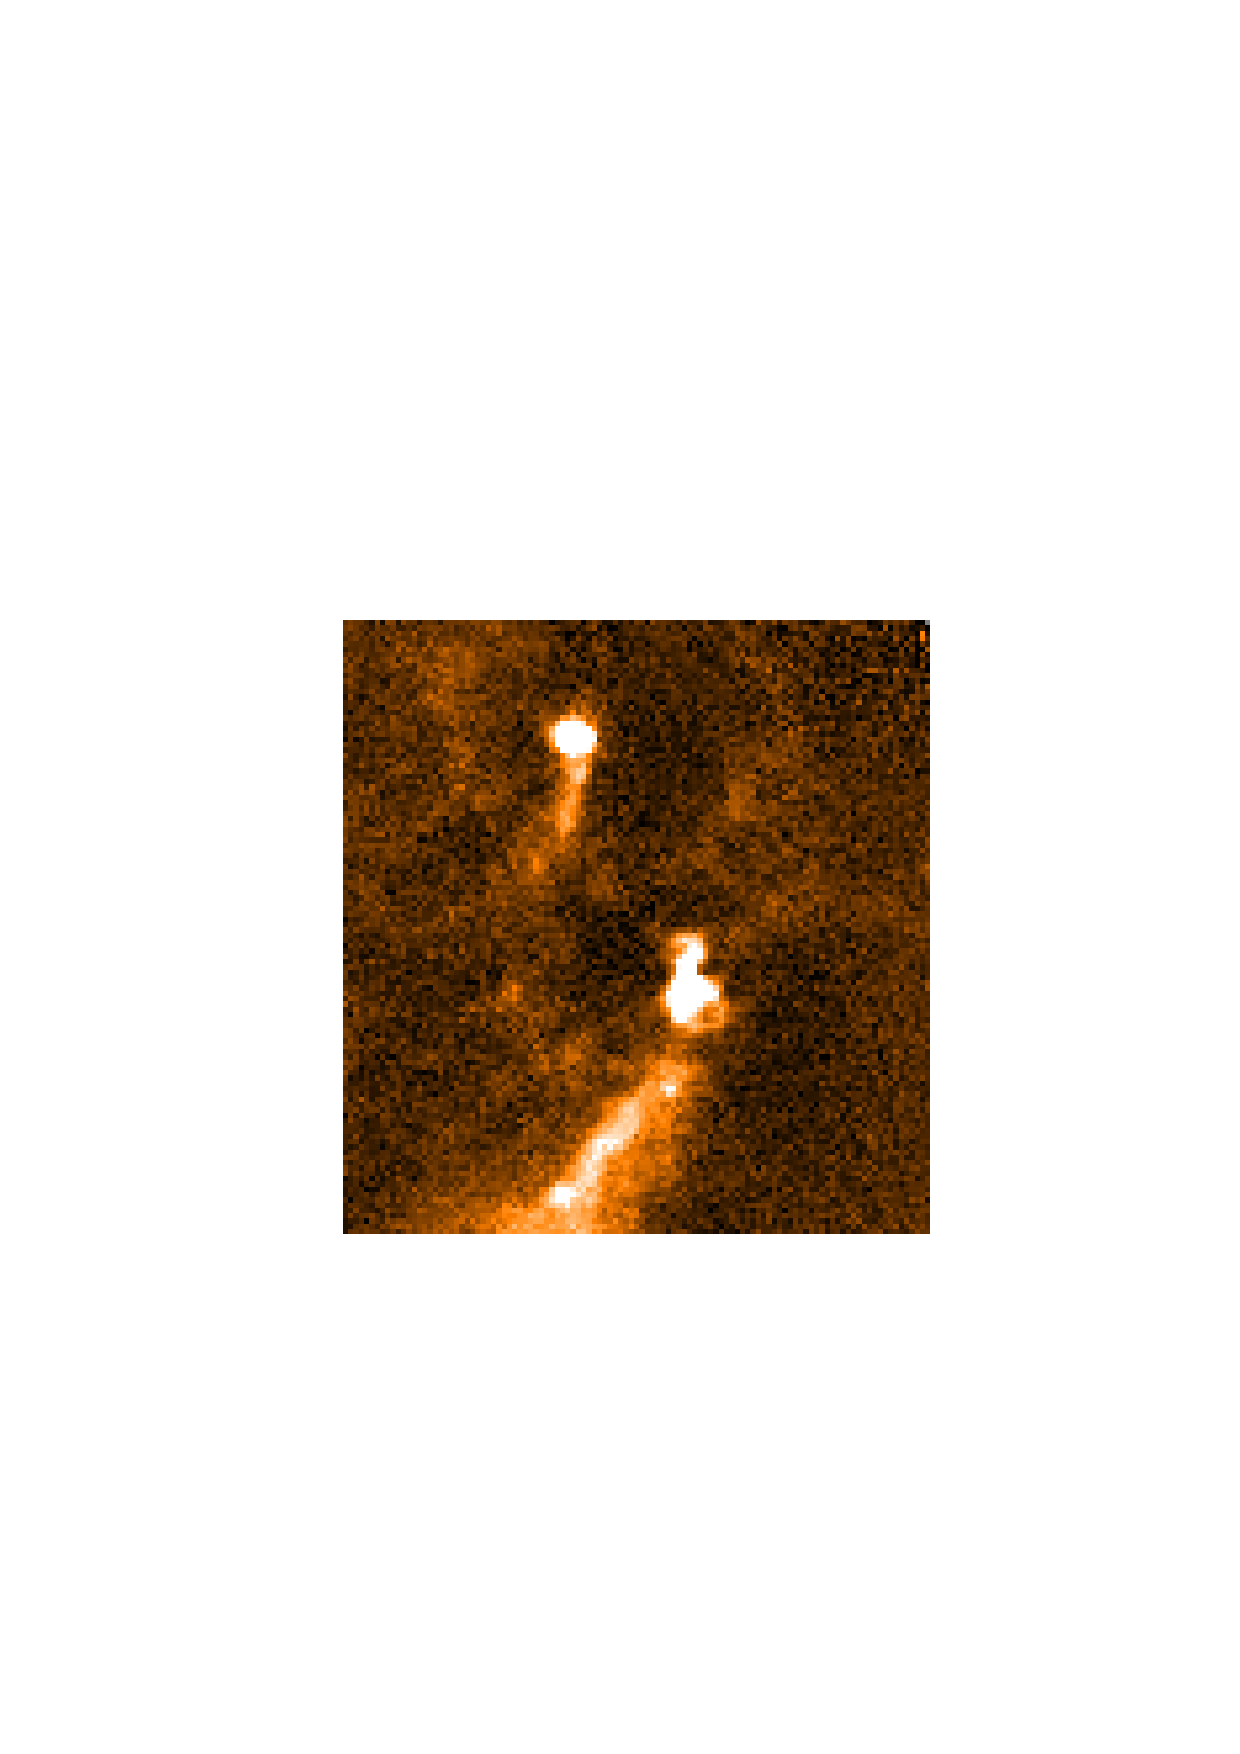
\includegraphics[width=0.7\linewidth]{sun258_itermap}
    \caption{Image reconstructed from simulated data using the
      \aparam{ITERATE} method. Note how the deep wells around bright
      sources are no longer present, and there are no cosmic ray
      spikes.}
    \label{fig:itermap}
  \end{center}
\end{figure}

Figure \ref{fig:itermap} shows an example of a map created from
simulated observations of an extended source using the `Iterate'
method. Compare this image with the map created from the same
observations using the `Rebin' method (see Figure
\ref{fig:rebinmap}).The dark regions around the bright sources have
disappeared and the cosmic ray spikes have been removed.


\subsubsection{Using the iterate method}

When using \makemap\ with the iterate option, the following parameters
and options have to applied:

\begin{itemize}
\item Create a configuration file, e.g.\ config.lis, containing all the
  required parameters listed in the form `keyword=value'. The
  configuration parameters are summarized in Table \ref{tab:dimmconfig}
  and the default values are shown in the third column. A default
  configuration file is located at
  \texttt{\$STARLINK/share/smurf/dimmconfig.lis}.
\item Set the \aparam{METHOD} parameter to \aparam{ITERATE}.
\item Set the correct pixel size for the observed wavelength using the
  \aparam{PIXSIZE} parameter.
\item If necessary, set the co-ordinate system using the \aparam{SYSTEM}
  parameter.
\end{itemize}

To make the map:
\begin{verbatim}
makemap in=^input.lis out=mapname method=iterate config=^config.lis \
        pixsize=value
\end{verbatim}


\subsubsection{Configuration parameters}

Table \ref{tab:dimmconfig} summarizes the configuration parameters
available for the model components used by the DIMM (see also detailed
comments for the \makemap\ task). The default values are shown in the
third column.

\begin{table}
\footnotesize
\centering
\begin{tabular}{llc}
\hline
Parameter        & Definition                                                         &  Default Value \\
(keyword)        &                                                                    & \\
\hline
                 & \multicolumn{2}{l}{\em General Options} \\
\hline
numiter          & Either give a positive number that equals the number of             & 5\\
                 & iterations, or give a negative number that equals the maximum       & \\
                 & number of iterations using chi squared ($\chi^2$) stopping criterion.& \\
chitol           & $\chi^2$ tolerance, requires $NOI$ model component. If the $\chi^2$ & $10^{-6}$\\
                 & difference $<1\times10^{-6}$, then make the current iteration the   & \\
                 & last iteration.                                                     & \\
varmapmethod     & Method of estimating variance map. If equal to zero, then use the   & 1 \\
                 & spread of values from the time-series (i.e. the raw data). If equal & \\
                 & to 1, then it samples the variance of data that land in each output & \\
                 & map pixel.                                                          & \\
maxlen           & If performing the iterations in memory, this is the maximum         &    0 \\
                 & length (seconds) for concatenated data. If equal to zero, then      & \\
                 & attempt to concatenate entire continuous chunks.                    & \\
modelorder       & Order in which to calculate DIMM model components.                  & (com,gai,ext,\\
                 &                                                                     &  ast,flt,noi)\\
exportndf        & An option to export DIMM model components as NDF files. It          & 0 (do not\\
                 & exports one file per model component, per subarray. Use this        & export as NDF\\
                 & option to view the values in these files. Can also      & files)\\
                 & specify list of components using modelorder syntax                  & \\
\hline
                 & \multicolumn{2}{l}{\em Pre-processing Data Cleaning Options} \\
\hline
pad              & Pad beginning and end of each chunk of data with this many samples          & 1000 \\
apod             & Apodize data at start and end over this many samples                & 1000 \\
zeropad          & Chooses how to pad - with zeros (1) or with artificial data (0)     & 0 \\
order            & Remove baseline polynomial of this order (0 = remove mean)          & 0 \\
badfrac          & If this fraction (or greater) of samples are bad, ignore entire bolometer            & 0.05 \\
flagstat         & Ignore data while telescope moving slower than this (arcsec/sec)    & 2 \\
dcthresh         & S/N threshold for detecting DC steps                                & -- \\
dcbox            & Sample length for measuring noise for DC step finder                & -- \\
spikethresh      & S/N threshold for detecting spikes                                  & -- \\
spikeiter        & iterations for spike $\sigma$-clipper (0=until convergence)         & 0 \\
filt\_edgehigh,  & Enter low- and high-pass frequency limits in hertz (Hz).            & -- \\
filt\_edgelow    & & \\
filt\_notchhigh, & Enter a range of high frequencies for filt\_notchhigh and a range   & -- \\
filt\_notchlow   & of low frequencies for filt\_notchlow to apply notch filters.       & \\
\hline
                 & \multicolumn{2}{l}{\em Control Model Component Calculation} \\
\hline
com.niter	 & Number of clipping iterations to use when finding common mode values & 1 \\
com.nsigma	 & Number of standard deviations at which to clip when finding common mode values & 3 \\
noi.spikethresh  & Additional despiking after each iteration, within the $NOI$         & 10 \\
                 & calculation.                                                        & \\
noi.spikeiter    & Additional despiking after each iteration, within the $NOI$         & 0 \\
                 & calculation.                                                        & \\
flt.filt\_edgehigh,  & Iterative filtering using $FLT$ model (see flt\_* above).       & 0.2 \\
flt.filt\_edgelow    &                                                                 & 20 \\
flt.filt\_notchhigh, &                                                                 & -- \\
flt.filt\_notchlow   &                                                                 & -- \\
ext.tausrc       & Source of opacity data: water vapour monitor (WVMRAW),              & WVMRAW \\
                 & $\tau_\mathrm{CSO}$ (CSOTAU), or explicit value for filter (FILTERTAU). & \\
ext.taumethod    & Airmass calculation: full (separate value for each detector each    & ADAPTIVE \\
                 & timeslice), quick (single airmass all detectors each timeslice), or & \\
                 & adaptive (decide dynamically to use full or quick).                 & \\
ext.csotau       & Value of zenith $\tau_\mathrm{CSO}$ if ext.tausrc=CSOTAU.            & -- \\
ext.filtertau    & Value of zenith optical depth for filter if ext.tausrc=FILTERTAU    & -- \\
\hline
\hline
\end{tabular}
\normalsize
\caption{Default parameters for the DIMM configuration file}
\label{tab:dimmconfig}
\end{table}

\section{\xlabel{simulator}SCUBA-2 Simulator\label{se:sc2sim}}

\SMURF\ has the capability to produce simulated data from SCUBA-2 with
the \sctwosim\ task. The simulator samples an input astronomical image
in the presence of a model atmosphere and other sources of noise.
Output files are written in the same format as real data from SCUBA-2
with complete flatfield, WVM, WCS and JCMT state structure
information. These files can be processed with other \SMURF\
tasks. Model atmospheres may be generated with the \skynoise\ task.

The simulator supports the primary observing modes: DREAM, STARE and
SCAN along with FLATFIELD, POINTING and FOCUS
observations. Rudimentary support exists for the SCUBA-2 polarimeter
though this is untested. Instrument apertures may be set (offsets
which adjust the tracking position to a specific subarray), and
microsteps (small offsets from the tracking position) are fully
supported. Simulating the motion of the major Solar System bodies
(Venus, the Moon, Mars, Jupiter, Saturn, Uranus and Neptune) is
supported.

For SCAN observations, the simulator has two modes controlled by the
\texttt{SIMTYPE} parameter. A \texttt{FULL} simulation generates
simulated complete astronomical data including the effect of the
atmosphere. A \texttt{WEIGHTS} simulation generates data which may be
used to assess areal coverage and `hit' density (i.e.\ the number of
times a point on the sky is observed) for different mapping strategies
or the impact of non-working bolometers. Several different scanning
models are supported: boustrophedon (conventional back-and-forth
raster scan), two variations of `pong' (or box-scan) with either
sharp or gentle turnarounds and a lissajous pattern. [REF TO ANA SCAN DOC]

\subsection{\xlabel{simuse}Simulator workflow\label{se:simuse}}

The simulator requires some preparatory work before data can be
simulated. The basic procedure is outlined below:
\begin{itemize}
\item Obtain an astronomical sky image;
\item Calculate a model atmosphere;
\item Calculate a flatfield solution;
\item Decide on simulation parameters;
\item Run simulation.
\end{itemize}
It is not necessary to recalculate a model atmosphere or flatfield
solution for every simulation, even for different input sky images.

Example files are installed as part of \SMURF\ and may be found in the
\texttt{\$STARLINK\_DIR/share/smurf} directory. An explanation may be
found in the \texttt{README} file in that directory.

\subsubsection{Astronomical image}

The astronomical image may be any suitable image, provided it has WCS
information. It should be as large as the size of the map to be
made. The WCS is used unless the source is a moving object (listed
above). The image must be an NDF. It is recommended that the image
pixel scale be set to be much less than the likely output map pixel
spacing (typically 3 arcsec at 850 $\mu$m, 1 arcsec at 450 $\mu$m) to
avoid imaging and sampling artefacts.

\subsubsection{Model atmosphere}

The model atmosphere is calculated with the \skynoise\ task. The
atmosphere is modelled as a Kolmogorov turbulent thin-screen
\cite{sc2ana002} with a characteristic turnover frequency and scaling
law. Different models may be generated for the same parameters using a
random number seed (specified or calculated internally using the
system clock). The parameters may be modified though the user should
be familiar with the details of this model of the atmosphere before
exploring the parameter space too widely.

The model atmosphere calculated is generic and may be used for
simulations at both 850 $\mu$m and 450 $\mu$m. The model is scaled
at the time of simulation according to the particular wavelength.

\subsubsection{Flatfield simulation}

Before a data simulation can take place, the flatfield solution for
each subarray must be calculated. This is achieved by specifying a
special observing mode called \texttt{heatrun} and running a
simulation.

The flatfield solution is written to a file using a naming scheme
which follows that for raw data. The convention is
\verb+s[4|8][a-d]heatYYYYMMDD_NNNNN.sdf+ where \verb+s[4|8][a-d]+ is
the subarray name (e.g.\ \verb+s8a+), \verb+heat+ indicates a
flatfield observation, \verb+YYYYMMDD+ is the date of observation and
\verb+NNNNN+ is a zero-padded, 5-digit observation number.

The simulator relies on this naming scheme for reading the flatfield
information, and the files must be present in the current directory.

\subsubsection{Running the simulator}

The simulator has a large number of parameters which may be freely
adjusted. The list of parameters is divided between two groups:
simulation parameters (usually telescope- and instrument-specific); and
observation parameters (properties of the observation in
question). These are specified using the \texttt{SIMPAR} and
\texttt{OBSPAR} ADAM parameters to \sctwosim. For convenience, the
parameters are stored in plain text files and are passed in using the
\verb+^+ scheme mentioned above in Section \ref{se:files}. Example
input files for all major observing modes may be found in the
\texttt{\$STARLINK\_DIR/share/smurf} directory.

The main observation parameters (\texttt{OBSPAR}) of interest are the
RA/Dec of the source, wavelength, observing mode (\texttt{obsmode}),
observation date and duration of observation (which in the case of
SCAN observations, is determined by the size of the area to
map). Planets may be specified by name. The RA/Dec must match that in
the astronomical image. If the source is not above the horizon, the
simulator will exit with an error message. The date must be specified
as a UT modified Julian day number. As a point of reference,
20090701T00:00:00 corresponds to MJD 55013.

The main simulation parameters (\texttt{SIMPAR}) are the subarrays to
simulate data for, the names of the atmosphere model and astronomical
source files and the zenith opacity (at 225 GHz). The zenith opacty is
converted to a value at the appropriate wavelength using the empirical
relations derived for SCUBA by Archibald et al. (2002). Similar
relations for SCUBA-2 will be derived.

Data for all subarrays (at the specified wavelength) may be generated
in a single run. The size of the output files is governed by the
\texttt{MAXWRITE} parameter for \sctwosim\ which specifies the number
of samples to write per file. Multiple observations may be simulated
by setting the \texttt{OVERWRITE} parameter to \texttt{FALSE} (the
default behaviour is to overwrite existing files).

A word of caution. Since the data output from the simulator mimics the
real instrument, it is possible to generate many GB of data which may
take many minutes to hours of CPU time. The \sctwosim\ parameter
\texttt{SIMSTATS} tells the simulator to estimate the properties of
the simulation including the duration of the simulation, quantity of
data, memory requirements and CPU time. The results are printed to the
screen, allowing the user to modify the simulation parameters if
necessary.

\subsubsection{\xlabel{dreamsim}A note on DREAM simulations\label{se:dreamsim}}

For STARE simulations, the images are calculated at 1-second intervals
at the time the simulator is run and written to the output files. For
DREAM the images must be reconstructed after the simulation has
run. This means that the DREAM weights file must be calculated using
\dreamweights\ as desribed in Section \ref{se:dream}. Likewise, the
images are calculated using \dreamsolve.

\subsection{\xlabel{simdr}Processing simulated data\label{se:simdr}}

The processing of simulated data proceeds exactly as for real SCUBA-2
data and depends on the observing mode. See the respective workflows
in Sections \ref{se:dsworkflow} and \ref{se:scanworkflow} above. Note
that dark frames are not produced by the simulator and do not need to
be included in any processing (there is no drift in the model
bolometer response).

FOCUS observations are designed to be processed by the ORAC-DR
pipeline rather than \SMURF, as their analysis involves multiple
steps. POINTING observations are equivalent to short science
observations and should be processed in the same way.

\section{Acknowledgments}

The authors are grateful for the documentation written by Maria Kelly
on which the SCUBA-2 part of this SUN was originally based, and
Christa van Laerhoven for an earlier version. The SCUBA-2 simulator
code was originally written as a standalone application by Dennis
Kelly at the UK Astronomy Technology Centre and converted to a \SMURF\
task by Jen Balfour.

% End of main text

\begin{thebibliography}{}
\addcontentsline{toc}{section}{References}

\bibitem{archibald}
Archibald~E.~N., et~al., 2002, MNRAS, 336, 1

\bibitem{acsis}
Buckle~J.~V., et~al., 2009, MNRAS, 399, 1026

%\bibitem{sc2cook}
%Chapin~E.~L., 2009, \textit{The SMURF SCUBA-2 Data Analysis Cookbook},
%\xref{Starlink Cookbook 19}{sc19}{}

%\bibitem{kappa}
%Currie~M.~J., 1997, {\it KAPPA -- Kernel Application Package},
%\xref{Starlink User Note 95}{sun95}{}

%\bibitem{gaia}
%Draper~P.~W., 1997, {\it GAIA -- Graphical Astronomy and Image
%Analysis Tool},
%\xref{Starlink User Note 214}{sun214}{}

\bibitem{scuba2}
Holland~W.~S., et~al., 2006, Proc. SPIE, 6275, 45

\bibitem{jenness}
Jenness~T., et~al., 2002, MNRAS, 336, 14

\bibitem{sc2ic01}
Jenness~T., Gibb,~A., 2007, \textit{Data Acquisition/Data Reduction
  Pipeline Interface Control Document}, SCUBA-2 Data Reduction
document SC2/SOF/IC210/01

\bibitem{dream}
Le~Poole~R.~S., van~Someren~Greve~H.~W., 1998, Proc. SPIE, 3357, 638

\bibitem{sc2ana001}
Scott~D., 2003, {\it Map-making in different noise regimes}, SCUBA-2
  Data Reduction document SC2/ANA/S210/001

\bibitem{sc2ana006}
Scott~D., 2005, {\it Scan Mode Data Reduction Strategies for
  SCUBA-2}, SCUBA-2 Data Reduction document SC2/ANA/S210/006

\bibitem{sc2ana005}
Scott~D., Van Engelen~A., 2005, {\it Scan Mode Strategies for
  SCUBA-2}, SCUBA-2 Data Reduction document SC2/ANA/S210/005

\bibitem{sc2ana002}
Van Engelen~A., 2005, {\it Analysis of Atmospheric Emission using
  SHARC-II Data and Implications for the SCUBA-2 Simulator},
  SCUBA-2 Data Reduction document SC2/ANA/S210/002

\bibitem{sc2ana004}
Van Engelen~A., Scott~D., 2005, {\it A Correlation Study using SCUBA
  Data, with implications for SCUBA-2 data reduction},
  SCUBA-2 Data Reduction document SC2/ANA/S210/002

%\bibitem{ast}
%Warren-Smith~R.~F., Berry~D.~S., 2009, {\it AST -- A Library for
%  Handling World Coordinate Systems in Astronomy},
%\xref{Starlink User Note 211}{sun211}{}

%\bibitem{ndf}
%Warren-Smith~R.~F., Berry~D.~S., 2009,
%{\it NDF -- Routines for Accessing the Extensible N-Dimensional Data
%  Format},
%\xref{Starlink User Note 33}{sun33}{}

\end{thebibliography}

\section{Release Notes}

\subsection{kaulia}

Supports compressed SCUBA-2 data files taken since February 2011.

\begin{itemize}
\item CALCQU - a new command to create Q and U values from SCUBA-2
  fast-spinning polarimeter time-series data files.
\item MAKECUBE
\begin{itemize}
\item Now allows the spatial reference pixel in the output cube to be
  specified by the user.
\item Setting \texttt{TRIM=YES} now modifies any user-supplied
  \texttt{LBND}/\texttt{UBND} values to remove borders of bad pixels.
\end{itemize}
\item MAKEMAP
\begin{itemize}
\item The loading and flatfielding of raw data on multi-core systems
  is now faster.
\item The focal plane distortion model has been updated to cover the
  entire focal plane.
\item A new parameter (\texttt{TRIM}) has been added to allow borders
  of blank pixels to be removed from the output map.
\item A bug has been fixed so that a request to perform just one
  iteration (\texttt{numiter=1}) is honoured.
\end{itemize}
\end{itemize}

\subsection{namaka}

Major updates to SMURF to support SCUBA-2 data processing.

\begin{itemize}
\item Polynomial fitting to flatfield data is now the default.
\item Fast flatfield ramps are now supported. These are taken at the
  start of every observation.
\item New scripts: smas analyzes "short maps" to investigate high
  frequency seeing/pointing variations
\end{itemize}

\subsubsection{MAKEMAP (iterative)}

\begin{itemize}
\item Maps from small chunks of the time series can now be written
  out. Specify the ``shortmap'' parameter.
\item Typos in config parameters are now trapped and the defaults can
  be seen in file \texttt{smurf\_makemap.def} in
  \texttt{\$SMURF\_DIR}. The actual parameters that are used (the
  merge of the supplied dimmconfig and the defaults) are now stored in
  the history of the output map.
\item Enhanced common-mode removal algorithm which can now break the
  time series into smaller chunks.
\item Enhanced spike removal using a rolling median calculation
\item Enhanced step correction.
\item Output map now includes QUALITY flags to indicate areas that
  have been set to 0 by the map-maker.
\item The map-maker now reports the details of the flagging every iteration.
\item Config files have been re-written to include the standard config
  with explicit overrides. This makes it easier to see what is being
  changed.
\item Major improvement to the speed of calculating the world
  coordinates of every bolometer.
\item Correctly switch to the CSO tau fits header in the absence of WVM data.
\end{itemize}

\subsubsection{SC2CLEAN}

\begin{itemize}
\item The parameter DCBOX has been renamed DCFITBOX.
\item DCBAD and DCFLAGALL parameters have been removed.
\end{itemize}

\subsubsection{SC2FFT}

\begin{itemize}
\item Add NGOOD parameter.
\item Can now calculate an average power spectrum.
\end{itemize}

\subsubsection{STACKFRAMES}

\begin{itemize}
\item Fix some bugs associated with maps of different sizes and with
  missing metadata.
\item Propagate QUALITY properly.
\end{itemize}

\subsection{V1.0.0 (hawaiki)}

First official release supporting SCUBA-2 raw data (rather than simulated data).

\subsubsection*{New applications}
\begin{itemize}
\item New command CALCNOISE for calculating the noise properties of a SCUBA-2 observation.
\item New command COPYFLAT to copy a flatfield from one SCUBA-2 observation to another.
\item New command STACKFRAMES for taking a collection of 2-D images
  (eg noise images or responsivities) and placing them into a time
  series cube.
\end{itemize}

\subsubsection*{Modified applications}
\begin{itemize}
\item SC2FFT will now concatenate all related files before calculating the FFT.
\item MAKECUBE can now avoid generating very thin tiles when tiling is enabled.
\item MAKECUBE now uses offset sky co-ordinates in the output cube if,
  and only if, the input tracking system is (Az,El) or geocentric
  apparent (RA,Dec).
\item JCMTSTATE2CAT now calculates DRA and DDEC columns to indicate
  arcsecond offsets from base position. Additionally DAZ and DEL are
  now given as offsets from BASE rather than offsets from the first
  base position. For SCUBA-2 files JCMTSTATE2CAT will now optionally include
  MCE header information and will calculate the tau dynamically from the
  raw WVM data.
\end{itemize}

\subsection{V0.5.2 (nanahope)}

\subsubsection*{Global changes}
\begin{itemize}
\item Improve description of SCUBA-2 processing routines for Nanahope
  Starlink release.
\item A summary of input observations is now presented.
\item If an output file is derived from multiple observations the
  output FITS header will now include start and end information (such
  as date and airmass from the oldest observation and date and airmass
  from the newest observation).

\end{itemize}

\subsubsection*{New applications}
\begin{itemize}
  \item New command CALCRESP for calculating responsivities from
    flatfield solutions.
\end{itemize}

\subsubsection*{Modified applications}
\begin{itemize}
  \item MAKECUBE can now fix up most issues associated with older ACSIS data from 2006 and 2007.
  \item MAKECUBE output catalogues can now contain additional JCMTSTATE information by using the EXTRACOLS parameter.
  \item TIMESORT is now significantly faster.
  \item MAKECUBE, MAKEMAP and QLMAKEMAP are now multi-threaded by default on multi-processor machines.
  \item MAKECUBE now issues a warning message if WCS information implied by the RECEPPOS and FPLANEX/Y values in an input NDF is inconsistent.
  \item TIMESORT can now handle single time slice data cubes.
  \item Many enhancements to SCUBA-2 functionality including support for bad pixel masks and interpolated darks.
 \item jcmtstate2cat now reports AZ and EL as well as DAZ and DEL.
\end{itemize}

\subsubsection*{Bug Fixes}

\begin{itemize}
\item MAKECUBE formerly mis-interpreted non-zero instrument aperture (INSTAP) values in recent ACSIS data.
\item MAKECUBE now ignores input data values that have negative input Tsys values.
\item TIMESORT now sets the correct pixel origin in the output NDFs.
\end{itemize}

\newpage
\appendix
\begin{small}
\section{\xlabel{ap_summary}An Alphabetical Summary of SMURF Commands
\label{ap:summary}}
\begin{htmlonly}
\begin{description}
\end{htmlonly}

\menuitem{ACSIS\_INDEX}{
  Provide a listing of ACSIS data files in a directory.}
\menuitem{BADBOLOS}{
  Generate a map of random dead bolometers and store in extension of the input file.}
\menuitem{CALCDARK}{
 Calculate the 2d dark frame from a dark observation.}
\menuitem{CALCFLAT}{
 Calculate a flatfield solution.}
\menuitem{CALCNOISE}{
Calculate the noise properties of a SCUBA-2 observation.}
\menuitem{CALCQU}{
Calculate Q and U images from a set of SCUBA-2 time-series data files.}
\menuitem{CALCRESP}{
 Calculate bolometer responsivity from stored flatfield solution.}
\menuitem{COPYFLAT}{
Copy the flatfield solution from one SCUBA-2 observation to another.}
\menuitem{DREAMSOLVE}{
 DREAM solver.}
\menuitem{DREAMWEIGHTS}{
 DREAM weight matrix generation.}
\menuitem{DSUTILS}{
Utility functions for estimating focal plane distortions.}
\menuitem{DUMPOCSCFG}{
Retrieve OCS XML configuration used to generate the raw data.}
\menuitem{EXTINCTION}{
 Extinction correct SCUBA-2 data.}
\menuitem{FIXSTEPS}{
Fix DC steps in a supplied SCUBA-2 time-series NDF.}
\menuitem{FLATFIELD}{
 Flatfield SCUBA-2 data.}
\menuitem{GETTSYS}{
Retrieve TSYS (or TRX) from ACSIS data files.}
\menuitem{GSD2ACSIS}{
 Convert a GSD format DAS data file to an ACSIS format NDF. (beta test)}
\menuitem{GSDSHOW}{
 Display the contents of a GSD file's headers and arrays.}
\menuitem{IMPAZTEC}{
  Import AzTEC NETCDF files and produce SCUBA-2 format data files. (untested)}
\menuitem{JCMTSTATE2CAT}{
Dump JCMTSTATE information to ASCII table.}
\menuitem{MAKECUBE}{
 Regrid ACSIS spectra into a data cube.}
\menuitem{MAKEMAP}{
 Regrid SCUBA-2 data into a map.}
\menuitem{MCEHEAD2CAT}{
 Dump the MCE data header of SCUBA-2 files.}
\menuitem{RAWFIXMETA}{
 Report metadata issues with ACSIS data files.}
\menuitem{RAWPRESS}{
Compress raw data that have not previously been compressed. (test routine)}
\menuitem{RAWRECREATEWCS}{
Attempt to fix corrupt spectral metadata in ACSIS data.}
\menuitem{RAWREWRTSC2WCS}{
Attempt to fix corrupt WCS in raw SCUBA-2 data.}
\menuitem{RAWUNPRESS}{
Uncompress raw SCUBA-2 data.}
\menuitem{REMSKY}{
  Remove Sky signal from SCUBA-2 observations.}
\menuitem{SC2CLEAN}{
 Clean-up SCUBA-2 time series.}
\menuitem{SC2CONCAT}{
 Concatenate files from a single observation into a single file.}
\menuitem{SC2EXPANDMODEL}{
Expand a DIMM model component into a full time-series data cube.}
\menuitem{SC2FFT}{
 Perform a forward or inverse FFT on SCUBA-2 data.}
\menuitem{SC2FILTERMAP}{
Filter a 2-D map.}
\menuitem{SC2MAPFFT}{
Fourier transform 2-D maps.}
\menuitem{SC2PCA}{
Use principal component analysis to identify correlated SCUBA-2 signals.}
\menuitem{SC2SIM}{
SCUBA-2 simulator.}
\menuitem{SCANFIT}{
  Fit a sky signal to each SCUBA-2 scan.}
\menuitem{SCUBA2\_INDEX}{
  Provide a listing of SCUBA-2 data files in a directory.}
\menuitem{SKYNOISE}{
 Generate a simulated sky background.}
\menuitem{SMAS}{
  Analyse shortmaps from the map-maker.}
\menuitem{SMURFCOPY}{
Copy a 2d image out of a time series file.}
\menuitem{SMURFHELP}{
Give help about SMURF.}
\menuitem{STACKFRAMES}{
Stack multiple 2-d images into a 3d cube, optionally sorted by time.}
\menuitem{STARECALC}{
 Calculate a map from a STARE-mode observation.}
\menuitem{TIMESORT}{
 Re-order time slices in a raw data cube into increasing time.}
\menuitem{UNMAKECUBE}{
 Produce simulated time series data from a regridded ACSIS data cube.}
\menuitem{UNMAKEMAP}{
Produce simulated time-series data from a SCUBA-2 map.}
\begin{htmlonly}
\end{description}
\end{htmlonly}

\newpage
\section{\xlabel{ap_classified}Classified SMURF Commands
\label{ap:classified}}

\SMURF\ applications may be classified in terms of their
functions as follows.

{\large
\begin{center}
{\bf General Purpose}
\end{center}
}

\begin{description}
\classitem{DUMPOCSCFG}
Retrieve OCS XML configuration used to generate the raw data.
\classitem{JCMTSTATE2CAT}
Dump JCMTSTATE information to ASCII table.
\classitem{SMURFHELP}
Give help about SMURF.
\classitem{STACKFRAMES}
Stack multiple 2-d images into a 3d cube, optionally sorted by time.
\end{description}

{\large
\begin{center}
{\bf SCUBA-2 Data Processing}
\end{center}
}

\begin{description}
\classitem{CALCDARK}
 Calculate the 2d dark frame from a dark observation.
\classitem{CALCFLAT}
 Calculate a flatfield solution.
\classitem{CALCNOISE}
Calculate the noise properties of a SCUBA-2 observation.
\classitem{CALCQU}
Calculate Q and U images from a set of SCUBA-2 time-series data files.
\classitem{CALCRESP}
 Calculate bolometer responsivity from stored flatfield solution.
\classitem{COPYFLAT}
Copy the flatfield solution from one SCUBA-2 observation to another.
\classitem{DREAMSOLVE}
 DREAM solver.
\classitem{DREAMWEIGHTS}
 DREAM weight matrix generation.
\classitem{DSUTILS}
Utility functions for estimating focal plane distortions.
\classitem{EXTINCTION}
 Extinction correct SCUBA-2 data.
\classitem{FIXSTEPS}
Fix DC steps in a supplied SCUBA-2 time-series NDF.
\classitem{FLATFIELD}
 Flatfield SCUBA-2 data.
\classitem{MAKEMAP}
 Regrid SCUBA-2 data into a map.
\classitem{MCEHEAD2CAT}
 Dump the MCE data header of SCUBA-2 files.
\classitem{RAWPRESS}
  Compress raw data that have not previously been compressed. (test routine)
\classitem{RAWRECREATEWCS}
  Attempt to fix corrupt spectral metadata in ACSIS data.
\classitem{RAWREWRTSC2WCS}
  Attempt to fix corrupt WCS in raw SCUBA-2 data.
\classitem{RAWUNPRESS}
  Uncompress raw SCUBA-2 data.
\classitem{REMSKY}
  Remove Sky signal from SCUBA-2 observations.
\classitem{SC2CLEAN}
 Clean-up SCUBA-2 time series.
\classitem{SC2CONCAT}
 Concatenate files from a single observation into a single file.
\classitem{SC2EXPANDMODEL}
  Expand a DIMM model component into a full time-series data cube.
\classitem{SC2FFT}
 Perform a forward or inverse FFT on SCUBA-2 data.
\classitem{SC2FILTERMAP}
  Filter a 2-D map.
\classitem{SC2MAPFFT}
  Fourier transform 2-D maps.
\classitem{SC2PCA}
  Use principal component analysis to identify correlated SCUBA-2 signals.
\classitem{SCANFIT}
  Fit a sky signal to each SCUBA-2 scan.
\classitem{SCUBA2\_INDEX}
  Provide a listing of SCUBA-2 data files in a directory.
\classitem{SMAS}
  Analyse shortmaps from the map-maker.
\classitem{SMURFCOPY}
Copy a 2d image out of a time series file.
\classitem{STARECALC}
 Calculate a map from a STARE-mode observation.
\classitem{UNMAKEMAP}
  Produce simulated time-series data from a SCUBA-2 map.
\end{description}

{\large
\begin{center}
{\bf ACSIS Data Processing}
\end{center}
}

\begin{description}
\classitem{ACSIS\_INDEX}
  Provide a listing of ACSIS data files in a directory.
\classitem{GETTSYS}
Retrieve TSYS (or TRX) from ACSIS data files.
\classitem{MAKECUBE}
 Regrid ACSIS spectra into a data cube.
\classitem{RAWFIXMETA}
 Report metadata issues with ACSIS data files.
\classitem{TIMESORT}
 Re-order time slices in a raw data cube into increasing time.
\classitem{UNMAKECUBE}
 Produce simulated time series data from a regridded ACSIS data cube.
\end{description}

{\large
\begin{center}
{\bf Data Import}
\end{center}
}

\begin{description}
\classitem{GSD2ACSIS}
 Convert a GSD format DAS data file to an ACSIS format NDF. (beta test)
\classitem{GSDSHOW}
 Display the contents of a GSD file's headers and arrays.
\classitem{IMPAZTEC}
 Import AzTEC NETCDF files and produce SCUBA-2 format data files. (untested)
\end{description}

{\large
\begin{center}
{\bf SCUBA-2 Simulations}
\end{center}
}

\begin{description}
\classitem{BADBOLOS}
 Generate a map of random dead bolometers and add it as an NDF extension to the input file.
\classitem{SC2SIM}
SCUBA-2 simulator.
\classitem{SKYNOISE}
 Generate a simulated sky background.
\end{description}

\end{small}

\section{\xlabel{ap_full}Specifications of SMURF Applications\label{ap:full}}

The following pages describe all the SMURF commands in detail. Default
values for parameters are quoted in square brackets. Empty brackets
indicate a dynamic default will be calculated and inserted at run
time. Parameters for which an array should be supplied (or are
returned) are shown with parentheses after the parameter name. A
number within those parentheses indicates the size of the array.

\subsection{ADAM routines}

\input{../../libsmurf/smurfmon}
\clearpage
\subsection{Scripts}

%% These are currently generated manually

\sstroutine{
  ACSIS\_INDEX
}{
  Provide a listing of ACSIS data files in a directory
}{
  \sstdescription{
    Reads ACSIS observation files in a directory and creates an
    index. Standard JCMT directory layout is supported.
  }
  \sstusage{
    acsis\_index   [-v | -h | -d | -o] [-a] [-c] [-e] [-f] [-t/T -r/R -s/S]
         [datadir]
  }
  \sstparameters{
    \sstsubsection{
      $-$all
    }{
      Print information on all files even if the headers are identical. For example,
      include multiple subbands (subsystems) and sub-scans.
    }
    \sstsubsection{
      $-$debug
    }{
      Print debugging information.
    }
    \sstsubsection{
      $-$extended
    }{
      Print extended lines. Can add AZ, EL, pointing offsets and bandwidth.
    }
    \sstsubsection{
      $-$force
    }{
      Force a subdirectory search. If no files are found in the
      directory itself, as would be the case for a raw data tree, the
      program will automatically search subdirecties. This option
      forces the subdirectory search.
    }
     \sstsubsection{
       $-$help
      }{
        Print help information.
      }
      \sstsubsection{
        $-$version
       }{
         Print version information.
       }
       \sstsubsection{
         $-$man
       }{
         Print the full documentation to STDOUT.
       }
       \sstsubsection{
         $-$ocscfg
       }{
         Print the OCS configuration XML file.
       }
       \sstsubsection{
         $-$cal
       }{
         Only print calibration observations.
       }
       \sstsubsection{
         $-$skip
       }{
         Skip observation information when printing Tsys or Trx
       }
       \sstsubsection{
         $-$stdev
       }{
         Include the standard deviation when printing Tsys or Trx.
       }
       \sstsubsection{
         $-$trx
       }{
         Print median receiver temperature.
       }
       \sstsubsection{
         $-$tsys
       }{
         Print median system temperature.
       }

  }
  \sstnotes{
    The primary argument is the data directory to index. If a \texttt{yyyymmdd} string is
    given it will default to the ACSIS data for the specified data unless
    there is a local subdirectory named \texttt{yyyymmdd}. Will default to the value of the
    \textsc{\$datadir} environment variable if set.
  }
  \sstdiytopic{
    Related Applications
  }{
    SMURF: SCUBA2\_INDEX, GETTSYS
  }
}

\clearpage
\sstroutine{
   DUMPOCSCFG
}{
   Retrieve OCS configuration XML from data file.
}{
  \sstdescription{
Searches for the OCS configuration in the file (if present) and writes
it to standard output. If the configuration is not present in the file
(older data will not contain it) the OCS configuration name is
retrieved and an attempt made to locate the file on the file system
(only valid at JAC).
 }
 \sstusage{
  dumpocscfg a20070105\_00050\_01\_0001.sdf
 }
  \sstparameters{
     \sstsubsection{
        $-$help
      }{
            Print help information.
      }
      \sstsubsection{
         $-$version
       }{
            Print version information.
       }
       \sstsubsection{
         $-$man
       }{
            Print the full documentation to STDOUT.
       }
  }

}

\clearpage
\sstroutine{
  GETTSYS
}{
  Get system temperature information from ACSIS data
}{
  \sstdescription{
Simple program to list TSYS or TRX information for receptors from an ACSIS data file. Optionally, calculates statistics.

  }
  \sstusage{
  gettsys --statistics a20070105\_00050\_01\_0001.sdf

  gettsys -trx --receptor h10 a20070105\_00050\_01\_0001.sdf
  }
 \sstparameters{
     \sstsubsection{
        $-$help
      }{
            Print help information.
      }
      \sstsubsection{
         $-$version
       }{
            Print version information.
       }
       \sstsubsection{
         $-$man
       }{
            Print the full documentation to STDOUT.
       }
   \sstsubsection{
      $-$trx
    }{
     Lists all TRX values for each receptor instead of TSYS.
    }
    \sstsubsection{
         $-$receptor
     }{
       Only report information for the current receptor.
    }
   \sstsubsection{
      $-$statistics
    }{
Report statistics in addition to the values. For tabular
form, the statistics are included at the end of the table
as additional lines of median, mean and standard deviation.
   }

  }

}

\clearpage

\sstroutine{
   JCMTSTATE2CAT
}{
   convert JCMT state structure into TST format
}{
   \sstdescription{
      Reads a set of SCUBA-2 or ACSIS files and writes a catalogue of
      the state information to standard out. The output file is in TST
      format and can be read into the TOPCAT application (but may
      require that TOPCAT is told explicitly that the catalogue is in
      TST format, e.g. with the {\tt "}-f tst{\tt "} command line option).

      This information includes the telescope pointing position (Actual,
      Demand and Base) in both the tracking system and AZEL coordinate
      frames, jiggle patterns, telescope row/offset index amongst
      others.
   }
  \sstusage{
      jcmtstate2cat *.sdf > catalogue.tst

      topcat -f tst catalogue.tst
   }
  \sstparameters{
     \sstsubsection{
        $-$help
      }{
            Print help information.
      }
      \sstsubsection{
         $-$version
       }{
            Print version information.
       }
       \sstsubsection{
         $-$man
       }{
            Print the full documentation to STDOUT.
       }
      \sstsubsection{
         $-$$-$with$-$mce
       }{
            Include SCUBA-2 MCE information in output table. This adds a lot of data to
            the output files and much of it is constant for the observation. Default
            is not to add this option. This option only works for data prior to summer
            of 2010 (which essentially means S2SRO data). After that date MCE data
            is written in a different form and is not supported. For modern data
            use the separate MCEHEAD2CAT command.
      }
   }
   \sstnotes{

    Additional derived columns are included in addition to those stored
    directly in the JCMTSTATE extension. All telescope values include
    a correction for motion of the secondary mirror.

    \sstitemlist{

      \sstitem \texttt{RA/DEC}

      Tracking coordinates in degrees. The columns will have the same name
      even if the telescope was tracking in GALACTIC.

      \sstitem \texttt{DRA/DDEC}

      Tracking offsets from the base position in arcsec.

      \sstitem \texttt{AZ/EL}

      Azimuth and elevation in degrees. Calculated directly from JCMTSTATE
      without being converted to RA/Dec.

      \sstitem \texttt{DAZ/DEL}

      Azimuth and elevation offsets from the base position in arcsec.

      \sstitem \texttt{TELSPEED}

      Instantaneous telescope speed in arcsec/sec.

      \sstitem \texttt{WVMTAU}

      Zenith 225 GHz opacity derived from the water vapor radiometer.

      \sstitem \texttt{PWVZEN}

      Precipitable water vapor at the zenith in mm.

      \sstitem \texttt{PWVLOS}

      Precipitable water vaport in the line of sight in mm.

    }

    Note that information from the ACSIS extension is not included at
    this time. This is partly because this extension can change in
    shape between observations.
    MCE header information is included for SCUBA-2 data files.
  }
}

\clearpage
\sstroutine{
  MCEHEAD2CAT
}{
  Convert SCUBA-2 MCE header information to TST format
}{
  \sstdescription{

    Reads a set of SCUBA-2 files and writes catalogues of the mcehead information
    to files. The output files are in TST format and can be read into the
    TOPCAT application (but may require that TOPCAT is told explicitly that
    the catalogue is in TST format, e.g. with the \texttt{-f tst} command line option).

    Multiple output files are created since the data are stored with
    different dimensionality. The \textit{root} name for the output files can be
    specified using the $-$\texttt{out} parameter (default: uses the  \texttt{s??ddmmyyyy\_nnnnn}
    part of the input file name or the basename of the filename if different).

    Output files (suffix: \texttt{tst}) are as follows:

    \sstitemlist{
      \sstitem \texttt{\_gen}:

      parameters that have a single value
      (includes the 10 values for \texttt{psc\_status\_psc} which
      don't fit the scheme)

      \sstitem \texttt{\_crd}:

      parameters that have 4 values

      \sstitem \texttt{\_col}:

      parameters that have 32 values
      (includes parameters that have 8 values since they
      always come in sets of 4).

      \sstitem \texttt{\_row}:

      parameters that have 41 values

    }
     If $-$\texttt{out} is used to specify the root output file name, out from all
     input files will be concatinated into a single set of output files.
  }

  \sstusage{
    mcehead2cat *.sdf

    mcehead2cat *.sdf -out="outroot" -item=par1,par2

    mcehead2cat *.sdf -item=\^list.in
  }
  \sstparameters{
    \sstsubsection{
      $-$help
    }{
      Print help information.
    }
    \sstsubsection{
      $-$version
    }{
      Print version information.
    }
    \sstsubsection{
      $-$man
    }{
      Print the full documentation to STDOUT.
    }
    \sstsubsection{
      $-$out
    }{
      Optional root name for the output files.
    }
    \sstsubsection{
      $-$items
    }{
      Optional comma-separated list of header items to print. Instead a filename
      listing the item names can be given as \texttt{-item=\^file}. The format of the
      file is the desired list of item names with one item per line.
    }
  }

  \sstnotes{
    For SCUBA-2 raw files, the program will only process the first file of
    any observation and skip all others. This is because the MCE
    configuration is only updated at the start of an observation. Assuming
    there are 10 observations for the night:

    \texttt{mcehead2cat /jcmtdata/raw/scuba2/s4a/20110524/*/*.sdf }

    will only process 10 files, not all x-nr sdf files that may be there.
    It will produce 10 sets of output files unless $-$\texttt{out} has been specified,
    in which case the mceheaders from the 10 files will be written to a
    single set of output files.

  }
}

\clearpage
\sstroutine{
  SCUBA2\_INDEX
}{
  Provide a listing of SCUBA-2 data files in a directory
}{
  \sstdescription{
    Reads ACSIS observation files in a directory and creates an
    index. Standard JCMT directory layout is supported.
  }
  \sstusage{
    scuba2\_index  [-v | -h | -d | -o] [-a] [-c] [-e] [-f] [datadir] [scuba2\_array]
  }
  \sstparameters{
    \sstsubsection{
      $-$all
    }{
      Print information on all files even if the headers are identical. For example,
      include multiple subbands (subsystems) and sub-scans.
    }
    \sstsubsection{
      $-$debug
    }{
      Print debugging information.
    }
    \sstsubsection{
      $-$extended
    }{
      Print extended lines. Can add AZ, EL, pointing offsets and bandwidth.
    }
    \sstsubsection{
      $-$force
    }{
      Force a subdirectory search. If no files are found in the
      directory itself, as would be the case for a raw data tree, the
      program will automatically search subdirecties. This option
      forces the subdirectory search.
    }
     \sstsubsection{
       $-$help
      }{
        Print help information.
      }
      \sstsubsection{
        $-$version
       }{
         Print version information.
       }
       \sstsubsection{
         $-$man
       }{
         Print the full documentation to STDOUT.
       }
       \sstsubsection{
         $-$ocscfg
       }{
         Print the OCS configuration XML file.
       }
       \sstsubsection{
         $-$cal
       }{
         Only print calibration observations.
       }
  }
  \sstnotes{
    The primary argument is the data directory to index. If a \texttt{yyyymmdd} string is
    given it will default to the SCUBA-2 data for the specified data unless
    there is a local subdirectory named \texttt{yyyymmdd}. Will default to the value of the
    \textsc{\$datadir} environment variable if set.

    This command can take a specific sub-array directory to index. Defaults to s8d.
  }
  \sstdiytopic{
    Related Applications
  }{
    SMURF: ACSIS\_INDEX, GETTSYS
  }
}

\clearpage
\sstroutine{
  SMAS
}{
  Short Map Analysis Script
}{
  \sstdescription{
    With the exception of Moon maps, each NDF is processed in the
    same way. The KAPPA:PSF command is used to locate the accurate
    source centre and fit it using an elliptical Gaussian-like
    model. The details of the model are then appended to an output
    text file as a new row.

    The resulting output catalogue has a row for every input NDF,
    and contains the following columns:

    \sstitemlist{
      \sstitem \texttt{TAI}: The MJD (in the TAI timescale) associated with the NDF
      \sstitem \texttt{UTC}: The UTC date and time string associated with the NDF
      \sstitem \texttt{SEQSTART} - RTS index number of first frame
      \sstitem \texttt{SEQEND} - RTS index number of last frame
      \sstitem \texttt{DLON}: The longitude offset at the centre of the source, in arc-seconds
      \sstitem \texttt{DLAT}: The latitude offset at the centre of the source, in arc-seconds
      \sstitem \texttt{AMP}: The peak value in the source
      \sstitem \texttt{SUM}: The total data sum in the source. This is the integral
      of the Gaussian-like model calculated by KAPPA:PSF
      \sstitem \texttt{FWHM}: The seeing-disc size: the full width at half maximum
      across the minor axis of the source (arc-seconds)
      \sstitem \texttt{AXISR}: The axis ratio of the source: the ratio of the major
      axis length to that of the minor axis.
      \sstitem \texttt{GAMMA}: The radial fall-off parameter of the source. A gamma
      of two would be a Gaussian.
      \sstitem \texttt{ORIENT}: The position angle (measured from north through east)
      of the major axis of the source, in degrees.
      \sstitem \texttt{NDF}: The path to the NDF
      \sstitem \texttt{ROW}: The row number for the bolometer (if known)
      \sstitem \texttt{COL}: The column number for the bolometer (if known)
      \sstitem \texttt{ARRAY}: The array name for the bolometer (if known)
    }

    For comparison, a set of extra columns is appended to these
    that give the source properties as calculated by KAPPA:BEAMFIT
    rather than KAPPA:PSF. These columns have the same names, but
    are prefixed by the letter B. Note, BEAMFIT assumes a gamma
    value of 2.0  (i.e. a pure Gaussian) and so there is no \texttt{BGAMMA}
    column in the output catalogue.

    The \texttt{SEQSTART} and \texttt{SEQEND} columns will be set to `null' if the
    supplied map does not contain these FITS headers.

    If the supplied data is for the Moon, then all the above is
    ignored and the output contains the following columns:

    \sstitemlist{
      \sstitem \texttt{SUM}: The integrated value within a 35 arc-minute aperture
      centred on (0,0)
      \sstitem \texttt{ROW}: The row number for the bolometer (if known)
      \sstitem \texttt{COL}: The column number for the bolometer (if known)
      \sstitem \texttt{ARRAY}: The array name for the bolometer (if known)
    }
  }
  \sstusage{
    smas [-a diam] [-b] [-e error] [-r perc] [-p] <in-list> <out-table> [<out-image>]
  }
  \sstparameters{
    \sstsubsection{
      $-$a
    }{
      Specifies that the catalogue \texttt{SUM} column values (the total
      data sum) should be the integrated data value within a
      circular aperture centred on the source peak position,
      with radius specified by ``diam'' (a numerical value in
      arc-seconds). This is calculated using KAPPA:APERADD.
      If this option is not supplied, the \texttt{SUM} value is the
      integrated value under the model source calculated by
      KAPPA:PSF. If ``diam'' is not supplied, defaults of 30 and
      15 are used for 850 and 450\,$\mu$m data respectively.
    }
    \sstsubsection{
      $-$b
    }{
      Specifies that the catalogue should contain only \texttt{ROW}, \texttt{COL} and
      \texttt{AMP} only. Using this option also implies the ``$-$p'' option.
      This reduces the run-time for script significantly.
    }
    \sstsubsection{
      $-$e
    }{
      Specifies the maximum allowed error (in arc-seconds) between the
      source position as determined by KAPPA:BEAMFIT and KAPPA:PSF.
      If the discrepancy in X or Y is greater than this value, then
      the shortmap or bolomap is not included in the returned catalogue
      or image. If the $-$e option is unspecified, then no sources are
      rejected. If no ``error'' value is supplied, a default of 1
      arc-second is used.
    }
    \sstsubsection{
      $-$p
    }{
      Specifies that the catalogue \texttt{AMP} column values (the peak
      value in the source) should be the maximum data value within
      a box of size 20 pixels centred on the expected source position.
      If this option is not supplied, the \texttt{AMP} value is the peak value
      of the model source calculated by KAPPA:PSF.
    }
    \sstsubsection{
      $-$r
    }{
      The following number (``perc'') specifies the minimum percentage of
      good pixel values in a small box around the expected source position.
      Sources that have insufficient good pixels in the box are reported
      and then ignored. If the ``-r'' option is not supplied (or is supplied
      without a "perc" value), a default of 95 is used.
    }
    \sstsubsection{
      $<$in-list$>$
    }{
      The path to an NDF holding a SCUBA-2 map of a point
      source (or Moon). Alternativelty, a text file containing the
      paths to one or more such NDFs can be supplied. If an NDF
      contains a \texttt{MORE.SMURF.SHORTMAPS} or \texttt{MORE.SMURF.BOLOMAPS}
      extension item, then the NDFs in the \texttt{SHORTMAPS} or \texttt{BOLOMAPS}
      array are used in place of the supplied NDF (\texttt{SHORTMAPS} is used
      in preference to \texttt{BOLOMAPS} if both are present). \textit{Note}, all the
      data must be for the same wavelength.
    }
    \sstsubsection{
      $<$out-table$>$
    }{
      The name of a text file in which to store a
      catalogue containing details of the source in each
      supplied map, as described below. This catalogue can
      be displayed and analysed using \texttt{topcat -f ascii
        $<$out-table$>$}.
    }
    \sstsubsection{
      $<$out-image$>$
    }{
      If supplied, and if the input data contains bolomaps,
      a 2D NDF containing the \texttt{SUM} (or \texttt{AMP} if the ``$-$b'' option is used)
      values for each bolometer is created with the name given by
      $<$out-image$>$. The FITS headers from the first input NDF are
      copied to the output NDF. If the supplied data contains values
      from more than one subarray, the name of the subarray is appended
      the end of each output NDF name.
    }
  }
}

\end{document}

